\documentclass[10pt,twoside]{report}
\usepackage{config/preamble}

\usepackage{csquotes}
\usepackage[sorting=none,giveninits=true]{biblatex}
\addbibresource{config/bibliography.bib}

\begin{document}

\pagenumbering{gobble}  % Do not number the first pages

% A title page generated from mojaPG
% 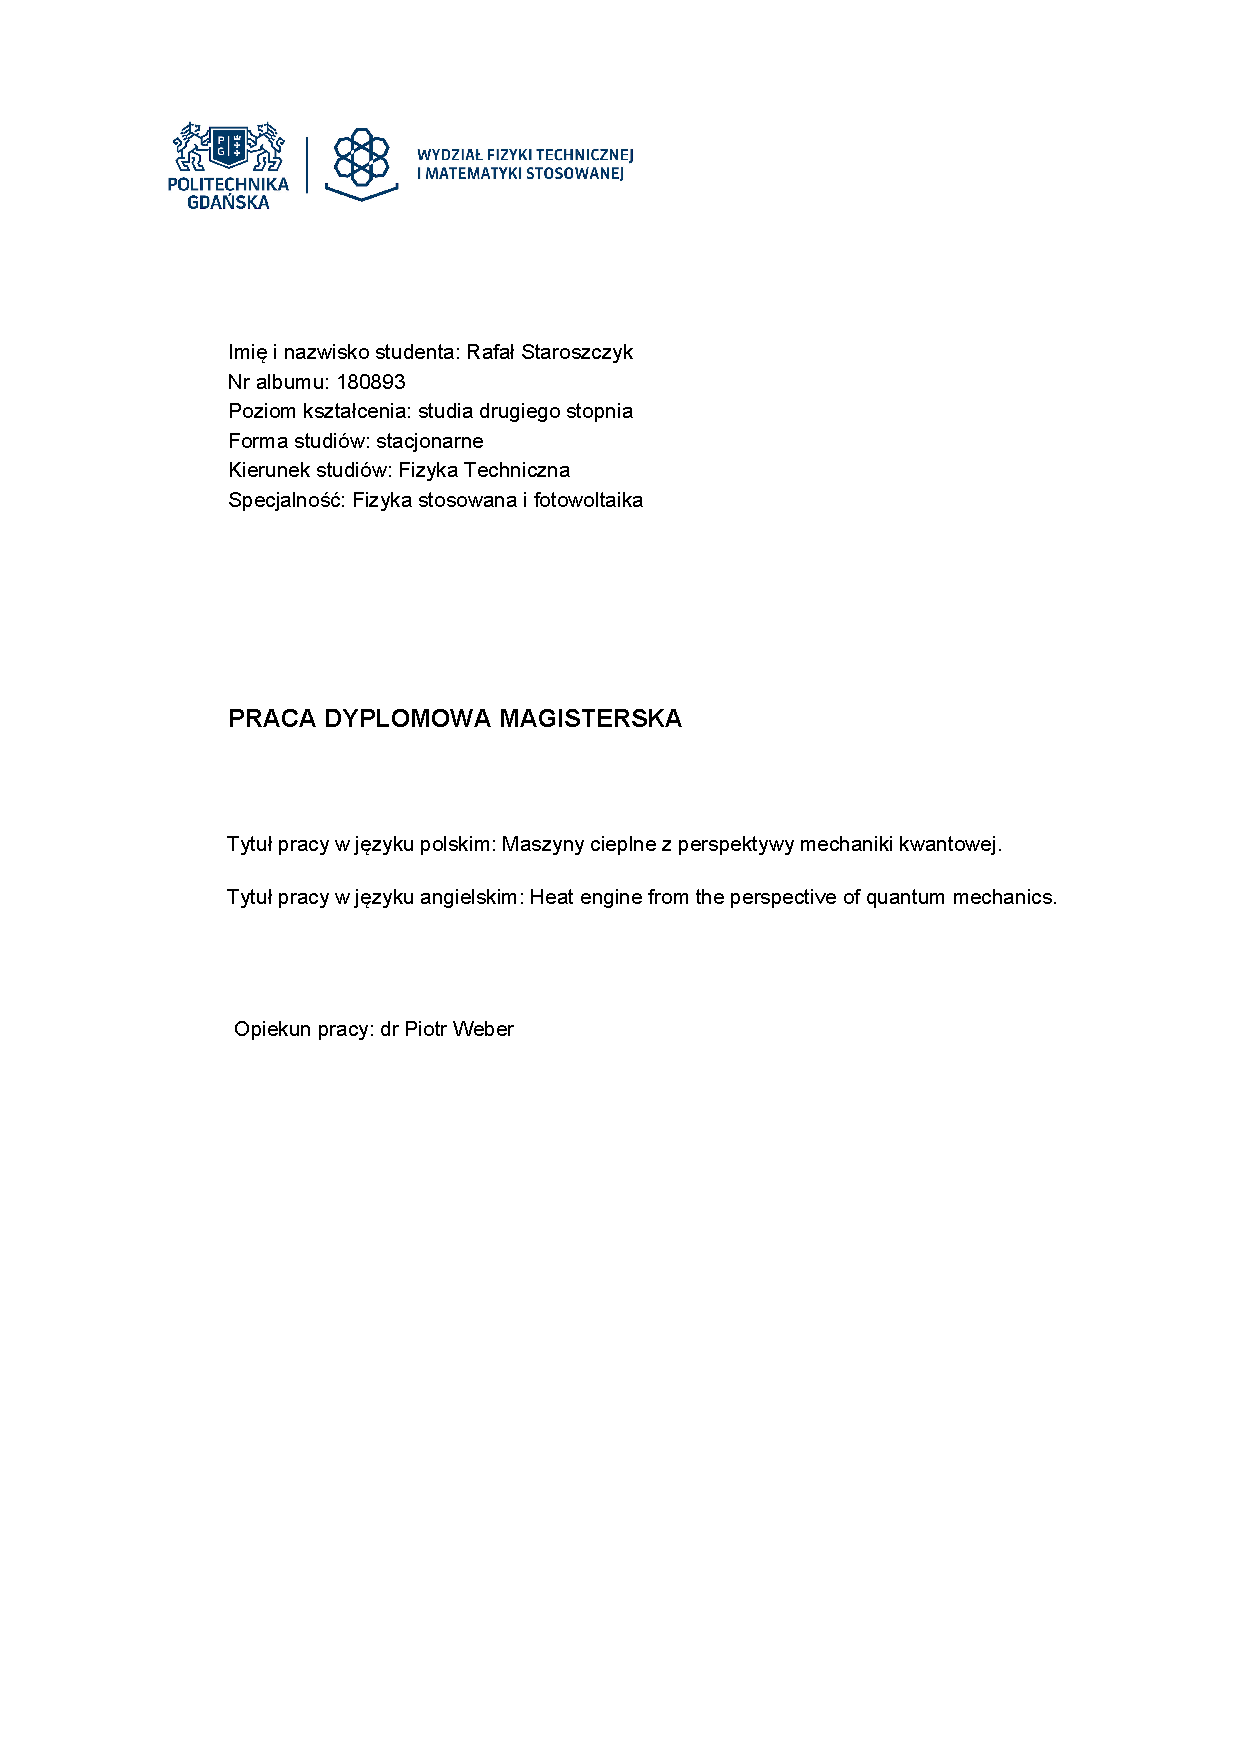
\includepdf[pages=-]{pdf/title-page.pdf}
% \null\newpage

% An author statement generated from mojaPG
% 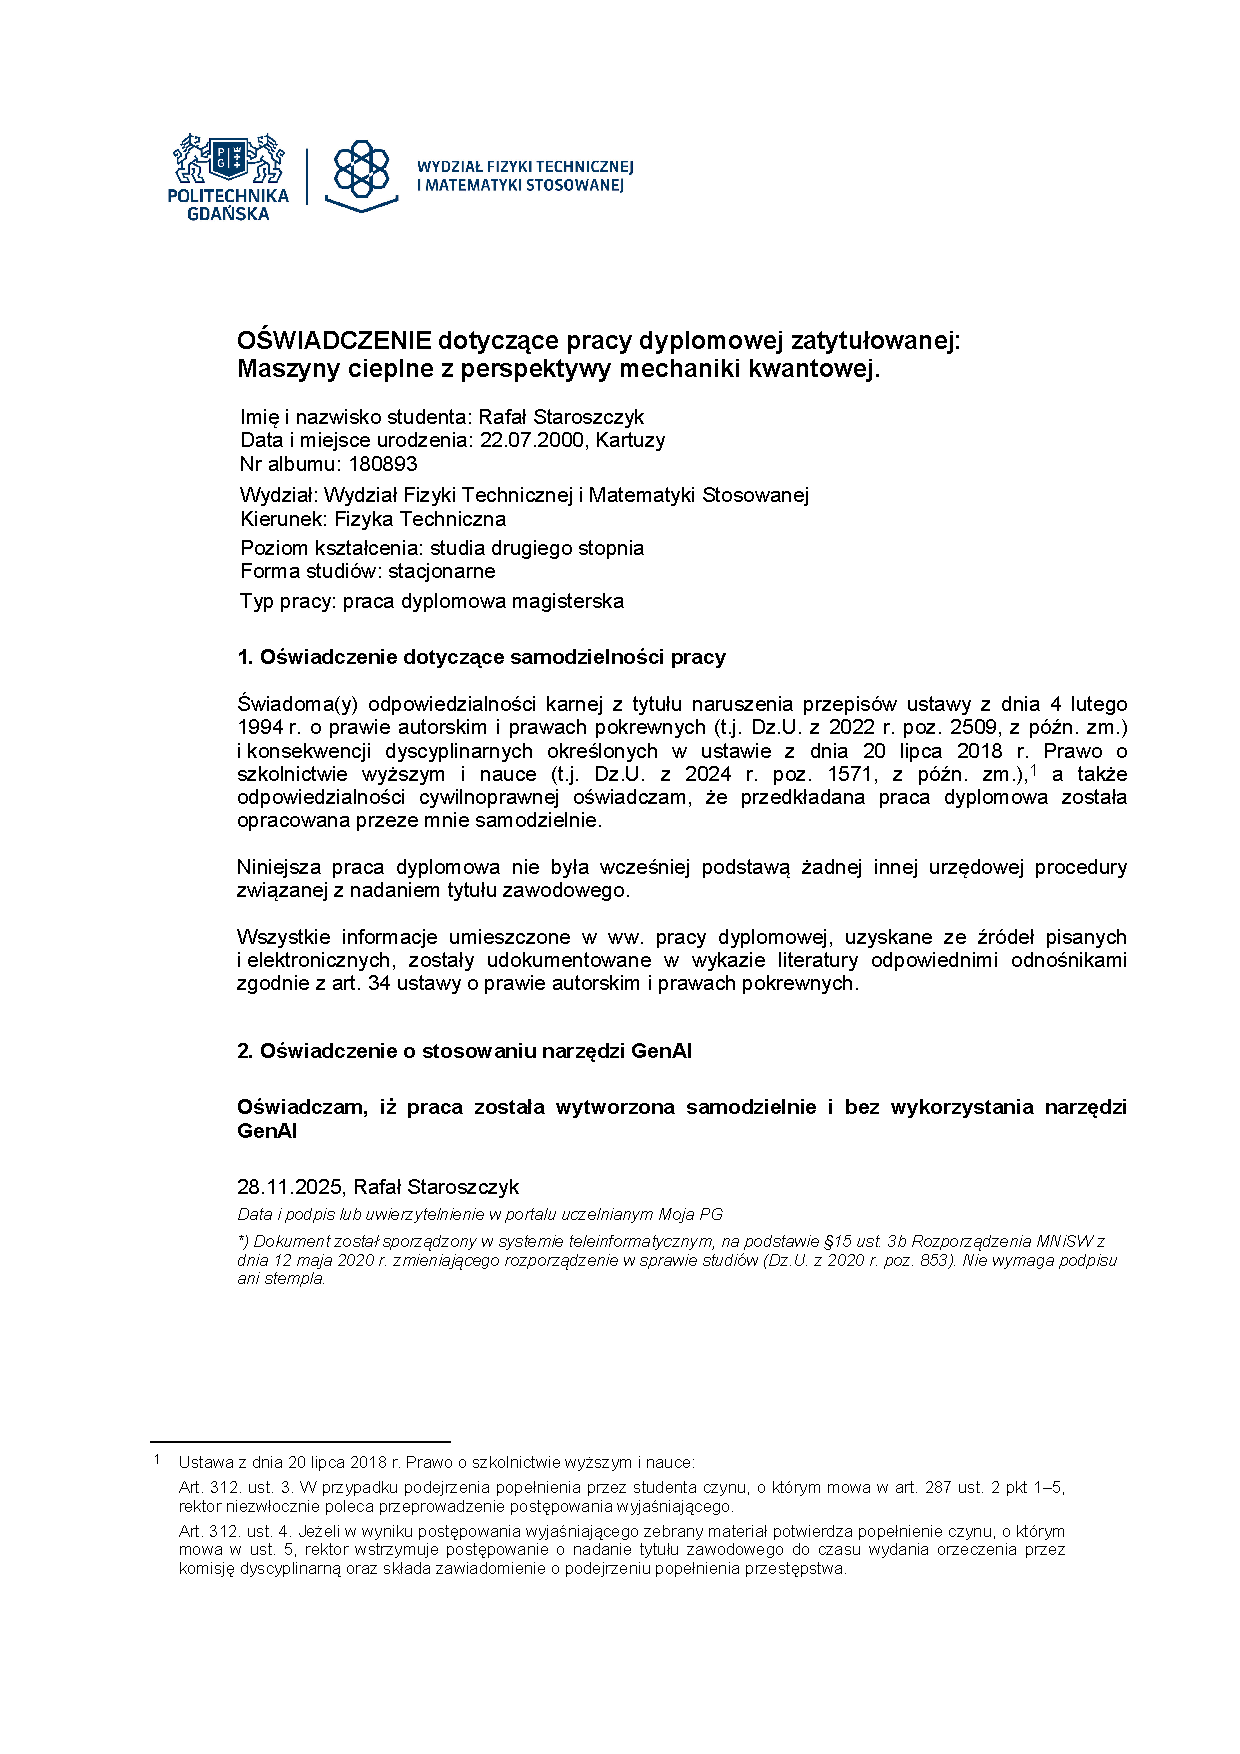
\includepdf[pages=-]{pdf/author-statement.pdf}
% \null\newpage

\chapter*{Streszczenie}

%Krótki wstęp.

%Część główna, która powinna być nieco dłuższa. Całe streszcznie powinno
%zająć około pół strony.

%Krótkie podsumowanie wniosków, wyników i ewentualnych proponowanych
%kolejnych kroków.

Silniki cieplne to maszyny konwertujące dostarczane do nich ciepło na pracę. W silnikach klasycznych czynnikiem roboczym najczęściej jest gaz, który czasem może zmienić stan na ciekły. W silnikach kwantowych natowmiast czynnikiem roboczym są układu kwantowe. Podczas pracy mogą być one w kontakcie ze zbiornikami ciepła o różnych temperaturach oraz w kontrolowanych warunkach zewnętrznych. Zmiana energii związana z samorzutną zmianą obsadzenia stanów kwantowych interpretowana jest jako ciepło, a jej zmiana poprzez kontrolowany parametr zewnętrzny jako praca. Silniki kwantowe dla pewnych cykli i czynników roboczych wykazują wyższe sprawności niż ich klasyczne odpowiedniki.

Kwantowe silniki cieplne są rezultatem połączenia analizy klasycznych silników cieplnych z układami kwantowymi jako czynnikiem roboczym. Pierwsze prace nad nimi rozpoczęły się od masera. Jest to układ kwantowy o przynajmniej trzech poziomach energetycznych. Jest on wzbudzany do stanu najwyższego, po czym następują dwa przejścia na kolejne stany niższe. Jedno z nich jest emisją wymuszoną, która jest analogiem wykonanej pracy.

W pracy przedstawiłem wyprowadzenie równań opisujących wybrane cykle termodynamiczne pracujące z wykorzystaniem dwóch układów kwantowych w roli czynnika roboczego: oscylatora harmonicznego oraz układu o spinie \(\inv{2}\). Wykonałem obliczenia numeryczne w celu znalezienia sprawności w punkcie maksymalnej mocy.

% Define 5-10 keywords which can describe what you're writing about
\bigskip
\noindent
\textbf{Słowa kluczowe:} silniki cieplne, termodynamika kwantowa

% Choose the field from the OECD list:
% https://en.wikipedia.org/wiki/Fields_of_Science_and_Technology
% With some research, you should find the whole list officially
% traslated into Polish.
% The below should be fine for PG ETI (informatyka)
\bigskip
\noindent
\textbf{Dziedzina nauki i techniki, zgodnie z wymogami OECD:}
nauki fizyczne

\newpage
\null\newpage

%\chapter*{Abstract}

\begin{otherlanguage}{english}

Heat engines are machines that convert added heat into work. In classical engines the most common working fluid is gas but in some cases it can change phase to a liquid. However, in quantum heat engines the working fluid is a quantum system. As the engine is running it can be in contact with heat baths at various temperatures and in controlled external conditions. The change of internal energy associated with spontaneous change of state populations is interpreted as heat and one associated with some external parameter is interpreted as work. For some combinations of thermodynamic cycles and working fluids the quantum heat engines achieve higher efficiency than the classical counterparts.

The field of quantum heat engines is the result of fusing classical heat engine analysis and quantum mechanical systems. First research came from thermodynamic description of a maser. It is a system with three energy states. Firstly it is pumped to the highest state and then it relaxes in two steps to the ground state. One of those transitions is a stimulated emission and is the work done on the enviroment.

In my thesis I derived the equations that describe selected thermodynamic cycles working with two quantum systes as working fluid: harmonic oscillator and spin \(\inv{2}\) system. I carried out numerical calculations to find efficiency of the engines is max power point.

%A short introduction.

%The main part which should be a bit longer. The whole abstract should take approximately a~half page.

%A short summary of the outcomes, results, and proposed next steps (if
%any).

% Define 5-10 keywords which can describe what you're writing about
\bigskip
\noindent
\textbf{Keywords:} heat engines, quantum thermodynamics

% Choose the field from the OECD list:
% https://en.wikipedia.org/wiki/Fields_of_Science_and_Technology
% The below should be fine for PG ETI (informatyka)
\bigskip
\noindent
\textbf{Field of science and technology in accordance with OECD
requirements:} physical sciences

\end{otherlanguage}

%\newpage
%\null\newpage

\pagenumbering{arabic}  % Start numbering on ToC
\tableofcontents

%\include{misc/list-of-symbols.tex}

% Include chapters one-by-one
%\include{chapters/01.tex}
\chapter{Termodynamika klasyczna}
% !TEX root = ../main.tex

\section{Silniki cieplne w termodynamice fenomenologicznej}
Silniki cieplne są maszynami konwertującymi cyklicznie dostarczane do nich ciepło na pracę mechaniczną, a czynnikiem roboczym jest płyn. Przebieg pełnego cyklu silnika cieplnego jest krzywą zamknięta na płaszczyźnie \(p\pab{V}\). Krzywa ta jest skierowana, co prowadzi do podzielenia cykli na prawobieżne i lewobieżne. Na rysunku \ref{fig:cykl_prawo_lewo} przedstawiono różnice pomiędzy cyklem prawobieżnym i lewobieżnym dla takiej samej krzywej zamkniętej. Podział ten odzwierciedla zasadnicze różnice w działaniu tych maszyn. Obiegi prawobieżne, których przykład przedstawiono na rysunku \ref{fig:cykl_prawobiezny}, wykonują pracę nad otoczeniem i są to silniki cieplne; obiegi lewobieżne, którego przykład przedstawiono na rysunku \ref{fig:cykl_lewobiezny}, powodują przepływ ciepła między zbiornikami kosztem wykonanej pracy nad układem i są to pompy ciepła. Pole ograniczone krzywą przebiegu reprezentuje wartość bezwzględną pracy objętościowej wykonanej w jednym cyklu.

Teoretyczny opis cykli termodynamicznych w przypadku ogólnym jest skomplikowany, ponieważ krzywa opisująca go może być dowolna. Aby je opisać wyróżnia się cykle wyidealizowane mające być przybliżeniem rzeczywistych przemian w silniku. Składają się one z elementarnych przemian termodynamicznych, które opisane są prostymi relacjami matematycznymi. Najważniejszym z cykli jest silnik Carnota, który ma duże znaczenie w termodynamice teoretycznej, a czynnikiem roboczym jest gaz doskonały.

\begin{figure}[H]
	\centering
	\begin{subfigure}{0.45\textwidth}
		\centering
		\input{figures/pv_silnik_prawo.tex}
		\caption{}
		\label{fig:cykl_prawobiezny}
	\end{subfigure}
	\begin{subfigure}{0.45\textwidth}
		\centering
		\tikzsetnextfilename{pv_silnik_lewo}
\begin{tikzpicture}
	\begin{axis}[width=\textwidth,
		xlabel=$V$,
		ylabel=$p$,
		axis x line=bottom,
		axis y line=middle,
		xmin=0,
		xmax=3,
		ymin=0,
		ymax=3,
		ticks=none,
		every axis x label/.style={at={(current axis.right of origin)},anchor=north east},
		every axis y label/.style={at={(current axis.above origin)},anchor=north east},
		declare function={
			centerx=1.5;
			centery=1.5;
			angle0=30;
			r = 1;
		}]
		\addplot[black,thick,->] ({centerx-r*cos(angle0)},{centery-r*sin(angle0)}) arc (180+angle0:270+angle0:r);
		\addplot[black,thick,->] ({centerx-r*sin(angle0)},{centery+r*cos(angle0)}) arc (90+angle0:180+angle0:r);
		\addplot[black,thick,->] ({centerx+r*cos(angle0)},{centery+r*sin(angle0)}) arc (angle0:90+angle0:r);
		\addplot[black,thick,->] ({centerx+r*sin(angle0)},{centery-r*cos(angle0)}) arc (-90+angle0:angle0:r);
	\end{axis}
\end{tikzpicture}

		\caption{}
		\label{fig:cykl_lewobiezny}
	\end{subfigure}
	\captionsetup{subrefformat=parens}
	\caption{Porównanie cyklu prawobieżnego \subref{fig:cykl_prawobiezny} i lewobieżnego \subref{fig:cykl_lewobiezny}.}
	\label{fig:cykl_prawo_lewo}
\end{figure}

W termodynamice technicznej powszechna jest konwencja, według której ciepło dostarczone z ciepłego zbiornika, odprowadzone do zimnego zbiornika oraz praca wykonana przez silnik są dodatnie \cite{b:huang_podstawy_fizyki_statystycznej}. Przepływy te zostały przedstawione na rysunku \ref{fig:konwencja_znakow_1}. Taki kierunek jest typowy podczas normalnej pracy. Tu mimo to użyta będzie konwencja powszechna w termodynamice statystycznej w celu ujednolicenia oznaczeń. W konwencji tej ciepła dostarczone do układu oraz praca wykonana nad układem mają znak dodatni. W przeciwnym przypadku mają one znak ujemny. Na rysunku \ref{fig:konwencja_znakow_2} przestawiono kierunku przepływu dodatniego.

\begin{figure}
	\centering
	\begin{subfigure}{0.45\textwidth}
		\centering
		\begin{tikzpicture}[x=0.5cm, y=0.5cm]
	\tikzmath{
		\tankwidth = 6;
		\tanksep = 5;
		\tankthickness = 1;
		\engwidth = 1;
		\engsep = 1;
		\radius = 2;
		\chansep = 1;
	}
	\draw[color=red, thick] (-\tankwidth, \tanksep) -- (\tankwidth, \tanksep);
	\draw[color=red, thick] (-\tankwidth, \tanksep) -- (-\tankwidth, \tanksep+\tankthickness);
	\draw[color=red, thick] (\tankwidth, \tanksep) -- (\tankwidth, \tanksep+\tankthickness);
	\fill[color=red, opacity=0.2] (-\tankwidth, \tanksep) rectangle (\tankwidth, \tanksep+\tankthickness);
	
	\draw[color=blue, thick] (-\tankwidth, -\tanksep) -- (\tankwidth, -\tanksep);
	\draw[color=blue, thick] (-\tankwidth, -\tanksep) -- (-\tankwidth, -\tanksep-\tankthickness);
	\draw[color=blue, thick] (\tankwidth, -\tanksep) -- (\tankwidth, -\tanksep-\tankthickness);
	\fill[color=blue, opacity=0.2] (-\tankwidth, -\tanksep) rectangle (\tankwidth, -\tanksep-\tankthickness);
	
	\draw[black] (-\engsep-\engwidth, -\tanksep) -- (-\engsep-\engwidth, \tanksep);
	\draw[black] (-\engsep+\engwidth, -\tanksep) -- (-\engsep+\engwidth, -\chansep-\radius);
	\draw[black] (-\engsep+\engwidth, \chansep+\radius) -- (-\engsep+\engwidth, \tanksep);
	\draw[black] (-\engsep+\engwidth, -\chansep-\radius) arc (180:90:\radius);
	\draw[black] (-\engsep+\engwidth, \chansep+\radius) arc (180:270:\radius);
	\node[anchor=east] at (-\engsep-\engwidth, 0.5*\tanksep)  {\(Q_h>0\)};
	\node[anchor=east] at (-\engsep-\engwidth, -0.5*\tanksep) {\(Q_c>0\)};
	\node[anchor=west] at (-\engsep+\engwidth+\radius, 0) {\(W>0\)};
	\draw[line width=0.3mm, -{Stealth[length=5mm, open]}] (-\engsep, 0.75*\tanksep) -- (-\engsep, 0.25*\tanksep);
	\draw[line width=0.3mm, -{Stealth[length=5mm, open]}] (-\engsep, -0.25*\tanksep) -- (-\engsep, -0.75*\tanksep);
	\draw[line width=0.3mm, -{Stealth[length=5mm, open]}] (-\engsep+\engwidth, 0) -- (-\engsep+\engwidth+\radius, 0);
\end{tikzpicture}
		\caption{}
		\label{fig:konwencja_znakow_1}
	\end{subfigure}
	\begin{subfigure}{0.45\textwidth}
		\centering
		\begin{tikzpicture}[x=0.5cm, y=0.5cm]
	\tikzmath{
		\tankwidth = 6;
		\tanksep = 5;
		\tankthickness = 1;
		\engwidth = 1;
		\engsep = 1;
		\radius = 2;
		\chansep = 1;
	}
	\draw[color=red, thick] (-\tankwidth, \tanksep) -- (\tankwidth, \tanksep);
	\draw[color=red, thick] (-\tankwidth, \tanksep) -- (-\tankwidth, \tanksep+\tankthickness);
	\draw[color=red, thick] (\tankwidth, \tanksep) -- (\tankwidth, \tanksep+\tankthickness);
	\fill[color=red, opacity=0.2] (-\tankwidth, \tanksep) rectangle (\tankwidth, \tanksep+\tankthickness);
	
	\draw[color=blue, thick] (-\tankwidth, -\tanksep) -- (\tankwidth, -\tanksep);
	\draw[color=blue, thick] (-\tankwidth, -\tanksep) -- (-\tankwidth, -\tanksep-\tankthickness);
	\draw[color=blue, thick] (\tankwidth, -\tanksep) -- (\tankwidth, -\tanksep-\tankthickness);
	\fill[color=blue, opacity=0.2] (-\tankwidth, -\tanksep) rectangle (\tankwidth, -\tanksep-\tankthickness);
	
	\draw[black] (-\engsep-\engwidth, -\tanksep) -- (-\engsep-\engwidth, \tanksep);
	\draw[black] (-\engsep+\engwidth, -\tanksep) -- (-\engsep+\engwidth, -\chansep-\radius);
	\draw[black] (-\engsep+\engwidth, \chansep+\radius) -- (-\engsep+\engwidth, \tanksep);
	\draw[black] (-\engsep+\engwidth, -\chansep-\radius) arc (180:90:\radius);
	\draw[black] (-\engsep+\engwidth, \chansep+\radius) arc (180:270:\radius);
	\node[anchor=east] at (-\engsep-\engwidth, 0.5*\tanksep) {\(\vab{Q_2}\)};
	\node[anchor=east] at (-\engsep-\engwidth, -0.5*\tanksep) {\(\vab{Q_1}\)};
	\node[anchor=west] at (-\engsep+\engwidth+\radius, 0) {\(\vab{W}\)};
	\draw[line width=0.5mm, -{Stealth[length=5mm, open]}] (-\engsep, 0.75*\tanksep) -- (-\engsep, 0.25*\tanksep);
	\draw[line width=0.5mm, -{Stealth[length=5mm, open]}] (-\engsep, -0.75*\tanksep) -- (-\engsep, -0.25*\tanksep);
	\draw[line width=0.5mm, -{Stealth[length=5mm, open]}] (-\engsep+\engwidth+\radius, 0) -- (-\engsep+\engwidth, 0);
\end{tikzpicture}
		\caption{}
		\label{fig:konwencja_znakow_2}
	\end{subfigure}
	\captionsetup{subrefformat=parens}
	\caption{Porównanie konwencji znaków: techniczna \subref{fig:konwencja_znakow_1} i statystyczna \subref{fig:konwencja_znakow_2}.}
\end{figure}

Z Pierwszej Zasady Termodynamiki wiadomo, że energia wewnętrzna \(U\) może być zmieniona jedynie poprzez wymianę ciepła \(Q\) lub wykonanie pracy nad układem \(W\) i ma formę:
\begin{equation*}
	\Delta U = Q + W,
\end{equation*}
co w formie różniczkowej ma postać \cite{b:huang_mechanika_statystyczna}:
\begin{equation}\label{eq:def_1zt}
	\d{U} = \idif{Q} + \idif{W},
\end{equation}
gdzie \(\dbar\) oznacza różniczkę niezupełną, czyli taką której całka zależy od drogi przemiany, wzdłuż której następuje całkowanie. W przeciwieństwie do niej \(\d{U}\) jest różniczką zupełną, co oznacza, że całka nie zależy od drogi, a \(U\) jest funkcją stanu. Całkując wyrażenie \eqref{eq:def_1zt} po jednym pełnym cyklu, pamiętając że \(\oint \d{U} = 0\), otrzymujemy:
\begin{equation}\label{eq:silnik_dU0}
	\oint \d{U} = 0 = \oint \idif{Q} + \oint \idif{W}, \quad\text{stąd}\quad
	-W = Q.
\end{equation}
Oznacza to, że suma ciepeł wymienionych między układem a otoczeniem jest równa pracy wykonanej przez układ \(-W\).

Silnik ma kontakt cieplny z dwoma zbiornikami o różnych temperaturach. Ciepło możemy rozdzielić na to dostarczone ze zbiornika ciepłego \(Q_h\) i na to oddane do zbiornika zimnego \(Q_c\):
\begin{equation}\label{eq:ciepla_w_silniku}
	Q = Q_h + Q_c.
\end{equation}
Zgodnie z równaniem \eqref{eq:silnik_dU0} praca wykonana jest równa:
\begin{equation}\label{eq:praca_w_silniku}
	-W = Q_h + Q_c.
\end{equation}
W cyklu prawobieżnym, w silnikach wykorzystujących gaz jako czynnik roboczy, praca wykonana \(W = - \oint p \d{V}\) jest kosztem ciepła \(Q_h\) pobranego ze zbiornika o temperaturze \(T_h\).

Parametrem opisujących efektywność przemiany dostarczonego do silnika ciepła na uzyskaną pracę jest sprawność silnika cieplnego:
\begin{equation}\label{eq:def_sprawnosc_silnika_W}
\eta = \frac{-W}{Q_h}.
\end{equation}
Biorąc pod uwagę relację \eqref{eq:praca_w_silniku} sprawność możemy zapisać poprzez ciepła \(Q_h\) i \(Q_c\):
\begin{equation}\label{eq:def_sprawnosc_silnika}
	 \eta = \frac{Q_h + Q_c}{Q_h} = 1 + \frac{Q_c}{Q_h}.
\end{equation}
Jest ona wielkością ważną zarówno w termodynamice teoretycznej jak i technicznej. W silnikach chcemy uzyskać jak największy zysk w postaci pracy jak najmniejszym kosztem w postaci dostarczonego ciepła \cite{b:pudlik_termodynamika}.

W analizie wyidealizowanych silników cieplnych rozważa się je jako serię elementarnych przemian: adiabatycznej (bez wymiany ciepła), izotermicznej (o stałej temperaturze czynnika roboczego), izobarycznej (o stałym ciśnieniu) oraz izochorycznej (o stałej objętości). Łącząc te przemiany w cykle zamknięte możemy otrzymać różnorodne cykle silników cieplnych o różnej liczbie przemian od 3, poprzez najpopularniejsze o 4 przemianach, i o większej ich liczbie. Przeanalizowane zostaną tu cykle: Carnota, Otta, Stirlinga.

\subsection{Cykl Carnota}
Silnik Carnota jest serią czterech przemian, w którym czynnikiem roboczym jest gaz doskonały spełniający równanie stanu:
\begin{equation}\label{eq:def_gaz_doskonaly}
	pV = nRT,
\end{equation}
gdzie \(p\) to ciśnienie gazu doskonałego, \(V\) -- objętość zajmowana przez ten gaz, \(n\) -- liczba moli tego gazu, \(R \approx \qty{8.314}{\joule / \kelvin / \mol}\) -- uniwersalna stała gazowa, \(T\) -- temperatura gazu.

\begin{figure}
	\centering
	\begin{tikzpicture}
	\begin{axis}[width=0.7\textwidth,
		xlabel=$V$,
		ylabel=$p$,
		axis x line=bottom,
		axis y line=middle,
		xmin=0,
		xmax=1.2,
		ymin=0,
		ymax=1.2,
		ticks=none,
		every axis x label/.style={at={(current axis.right of origin)},anchor=north east},
		every axis y label/.style={at={(current axis.above origin)},anchor=north east},
		declare function={
			r = 2;
			tau = 2;
			f = 3;
			kappa = 1 + 2/f;
			V1 = 1;
			V2 = 1/r;
			V3 = 1/r * tau^(-1/(kappa-1));
			V4 = tau^(-1/(kappa-1));
			p1 = 1/r * tau^(-kappa/(kappa-1));
			p2 = tau^(-kappa/(kappa-1));
			p3 = 1;
			p4 = 1/r;
		}]
		\addplot[mark=*] coordinates {(V1,p1)} node[anchor=south west]{$1$};
		\addplot[mark=*] coordinates {(V2,p2)} node[anchor=north east]{$2$};
		\addplot[mark=*] coordinates {(V3,p3)} node[anchor=south east]{$3$};
		\addplot[mark=*] coordinates {(V4,p4)} node[anchor=south west]{$4$};
		\addplot[domain=V2:V1] {1/r * tau^(-kappa/(kappa-1)) / x}             node [pos=0.3, below, sloped] {$T_c$};
		\addplot[domain=V3:V2] {1/r^kappa * tau^(-kappa/(kappa-1)) / x^kappa} node [pos=0.5, below, sloped] {$Q=0$};
		\addplot[domain=V3:V4] {1/r * tau^(-1/(kappa-1)) / x}                 node [pos=0.5, above, sloped] {$T_h$};
		\addplot[domain=V4:V1] {1/r * tau^(-kappa/(kappa-1)) / x^kappa}       node [pos=0.5, above, sloped] {$Q=0$};
		\draw[line width=0.3mm, -{Stealth[length=5mm, open]}] (0.4,0.7) node[anchor=south west]{$Q_{3-4}$} -- (0.3,0.6);
		\draw[line width=0.3mm, -{Stealth[length=5mm, open]}] (0.75,0.1) -- (0.75,0.025) node[anchor=west]{$Q_{1-2}$};
	\end{axis}
\end{tikzpicture}

	\caption{Wykres cyklu Carnota w obiegu prawobieżnym.}
	\label{fig:pv_silnik_carnot}
\end{figure}

Przemiany w cyklu Carnota zaprezentowane są na rysunku \ref{fig:pv_silnik_carnot}. Są to po kolei: sprężanie izotermiczne w temperaturze \(T_c\); sprężanie adiabatyczne, której skutkiem jest podniesienie temperatury do \(T_h\); rozprężanie izotermiczne w tej samej temperaturze; oraz rozprężanie adiabatyczne do temperatury początkowej. Każda z przemian silnika Carnota jest odwracalna, a więc i cały cykl jest odwracalny. Przemiany izotermiczne występują bez różnicy temperatur między czynnikiem roboczym a zbiornikiem cieplnym. Energia wewnętrzna gazu doskonałego zależy jedynie od temperatury \cite{b:kondepudi_prigogine_modern_thermodynamics}. Oznacza to, że podczas przemian izotermicznych \(\Delta U = 0\), a \(- W = Q\).

Silnik taki można uruchomić w drugą stronę. Spowoduje to zmianę znaków \(W\), \(Q_{3-4}\) oraz \(Q_{1-2}\) i w efekcie kosztem włożonej pracy pobrane zostanie ciepło \(Q_{1-2}\) z zimniejszego zbiornika o temperaturze \(T_c\) i oddanie ciepła \(Q_{3-4}\) do cieplejszego o temperaturze \(T_h\). Aby przemiana izotermiczna była odwracalna musi być nieskończenie powolna. Cykl ten jest więc nieosiągalny w rzeczywistości, ale ma duże znaczenie w teorii termodynamiki, ponieważ stanowi górną granicę dla sprawności silników cieplnych.

W silniku Carnota ciepła oddane do zbiornika o temperaturze \(T_c\) i dostarczone ze zbiornika o temperaturze \(T_h\) są równe odpowiednio:
\begin{gather*}
	Q_{1-2} = - W_{1-2} = \int_{V_1}^{V_2} p \d{V} = nRT_c \ln\pab{\frac{V_2}{V_1}}, \\
	Q_{3-4} = - W_{3-4} = \int_{V_3}^{V_4} p \d{V} = nRT_h \ln\pab{\frac{V_4}{V_3}},
\end{gather*}
gdzie \(V_1\), \(V_2\), \(V_3\) oraz \(V_4\) to objętości gazu w silniku w punktach oznaczonych na rysunku \ref{fig:pv_silnik_carnot}. Objętości te są powiązane ze sobą warunkami wynikającymi z przemian adiabatycznych \cite{b:pudlik_termodynamika}:
\begin{align*}
	p_{2}V_{2}^{\varkappa} &= p_{3}V_{3}^{\varkappa}, \\
	p_{1}V_{1}^{\varkappa} &= p_{4}V_{4}^{\varkappa},
\end{align*}
gdzie parametr \(\varkappa\) to wykładnik adiabaty zależny od użytego gazu. Parametr ten wyraża się przez ciepło molowe przy stałym ciśnieniu \(c_p\) i ciepło molowe przy stałej objętości \(c_V\) wzorem \(\varkappa = \frac{c_p}{c_V}\). Wykorzystując wzór \eqref{eq:def_gaz_doskonaly} możemy znaleźć:
\begin{equation*}
	\frac{V_1}{V_2} = \frac{V_4}{V_3}.
\end{equation*}
Sprawność silnika jest równa:
\begin{equation}\label{eq:sprawnosc_silnika_Carnota}
	\eta = 1 + \frac{Q_{1-2}}{Q_{3-4}} =
	1 + \frac{nRT_c \ln\pab{\frac{V_2}{V_1}}}{nRT_h \ln\pab{\frac{V_4}{V_3}}} =
	1 - \frac{T_c}{T_h}.
\end{equation}
Wzór ten pokazuje, że sprawność silnika Carnota jest funkcją jedynie stosunku temperatur zbiorników.

\subsection{Cykl Otto}
Cykl Otto składa się ze sprężania adiabatycznego (\(1 \rightarrow 2\)), podgrzania izochorycznej (\(2 \rightarrow 3\)), rozprężania adiabatycznego (\(3 \rightarrow 4\)) oraz ochłodzenia izochorycznego (\(4 \rightarrow 1\)). Przedstawiono go na rysunku \ref{fig:pv_silnik_otto}. Silnik ten pracuje pomiędzy dwoma zbiornikami o różnych temperaturach. Ciepło dostarczane jest ze zbiornika o temperaturze \(T_h\), a oddawane do zbiornika o temperaturze \(T_c\). Podczas pobierania ciepła ze zbiornika o temperaturze \(T_h\) czynnik roboczy znajduje się w temperaturze niższej niż \(T_h\). Natomiast podczas oddawania ciepła do drugiego zbiornika o temperaturze \(T_c\) znajduje się on w temperaturze od niego wyższej. W trakcie tych przemian temperatura zbiorników jest stała i przepływy ciepła nie mają na nie wpływu. Przemiany te zachodzą więc przy spadku temperatury na ściankach silnika, co czyni go nieodwracalnym. Zgodnie z \eqref{eq:praca_w_silniku} aby określić pracę wykonaną w cyklu należy znaleźć ciepło dostarczone oraz odprowadzone, co ma miejsce jedynie podczas przemian (\(2 \rightarrow 3\)) oraz (\(4 \rightarrow 1\)). W przemianie izochorycznej według wzoru \eqref{eq:def_1zt} ciepło to jest równe zmianie energii wewnętrznej i jest równe \cite{b:pudlik_termodynamika}:
\begin{equation}
	\idif{Q} = \pab{\pdv{U}{T}}_{V} \d{T} = n c_{V} \d{T},
\end{equation}
gdzie \(c_{V}\) to ciepło molowe dla stałej objętości, które dla gazu doskonałego jest parametrem niezależnym od temperatury. Całkując to wyrażenie podczas przemian otrzymujemy:
\begin{equation}\label{eq:otto_Q}
\begin{split}
	Q_{2-3} = n c_{V} \pab{T_3 - T_2}, \\
	Q_{4-1} = n c_{V} \pab{T_1 - T_4},
\end{split}
\end{equation}
gdzie temperatury \(T_1\), \(T_2\), \(T_3\) oraz \(T_4\) to temperatury w punktach oznaczonych na wykresie \ref{fig:pv_silnik_otto}. Sprawność tego cyklu wyraża się wzorem:
\begin{equation}
	\eta = 1 + \frac{Q_{2-3}}{Q_{4-1}} = 1 - \frac{T_3 - T_2}{T_4 - T_1}.
\end{equation}
Wzór ten jest zależny od temperatur, których nie kontrolujemy bezpośrednio. Należy go wyrazić poprzez inne wielkości.

\begin{figure}
	\centering
	\input{figures/pv_silnik_otto.tex}
	\caption{Wykres cyklu Otto w obiegu prawobieżnym.}
	\label{fig:pv_silnik_otto}
\end{figure}

Parametry gazu w przemianie adiabatycznej spełniają wyrażenia pomocnicze \cite{b:pudlik_termodynamika}:
\begin{equation}
\begin{split}
	p_{1}V_{1}^{\varkappa} &= p_{2}V_{2}^{\varkappa}, \\
	p_{4}V_{1}^{\varkappa} &= p_{3}V_{2}^{\varkappa}.
\end{split}
\end{equation}
Obie z powyższych równości możemy przekształcić, aby ciśnienia zależały od stosunku objętości:
\begin{equation*}
	\frac{p_2}{p_1} = \frac{p_3}{p_4} = \pab{\frac{V_1}{V_2}}^{\varkappa} = r^{\varkappa}.
\end{equation*}
Wykorzystując równanie stanu gazu doskonałego \eqref{eq:def_gaz_doskonaly} możemy znaleźć analogiczną formę zależną of temperatury i objętości:
\begin{equation}
\begin{split}
	T_{1}V_{1}^{\varkappa-1} &= T_{2}V_{2}^{\varkappa-1}, \\
	T_{4}V_{1}^{\varkappa-1} &= T_{3}V_{2}^{\varkappa-1}.
\end{split}
\end{equation}
Dzieląc stronami otrzymujemy stosunki temperatur. Podobnie jak wyżej możemy wyrazić stosunek temperatur też za pomocą współczynnika sprężenia:
\begin{gather}
	\frac{T_3}{T_2} = \frac{T_4}{T_1}, \\
	\frac{T_2}{T_1} = \frac{T_3}{T_4} = \pab{\frac{V_1}{V_2}}^{\varkappa-1} = r^{\varkappa-1} \label{eq:otto_stosunek_T}.
\end{gather}
Posługując się tymi wielkościami możemy wyrazić temperatury \(T_2\) i \(T_3\) poprzez \(T_1\), \(T_4\), \(r\) i \(\varkappa\):
\begin{gather}
	T_2 = T_1 r^{\varkappa-1}, \\
	T_3 = T_4 r^{\varkappa-1}.
\end{gather}
Podstawiając je do wzorów na pracę oraz sprawność otrzymujemy:
\begin{gather}
	- W = n c_V \pab{r^{\varkappa-1} - 1} \pab{T_4 - T_1}, \label{eq:parametry_otto_W} \\
	\eta = 1 - \inv{r^{\varkappa-1}}. \label{eq:parametry_otto_eta}
\end{gather}
Możemy zauważyć, że sprawność nie zależy od temperatury a jedynie od stopnia sprężenia \(r\), który jest parametrem mechanicznym danego silnika. Ponieważ \(\varkappa > 1\) sprawność rośnie wraz ze wzrostem stopnia sprężenia \(r\).

\subsection{Cykl Stirlinga}
Podobnie jak cykl Carnota i cykl Otto, cykl Stirlinga składa się z czterech przemian. Są to po kolei: sprężanie izotermiczne w temperaturze \(T_c\) (\(1 \rightarrow 2\)), podgrzewanie izochoryczne (\(2 \rightarrow 3\)), rozprężenie izotermiczne w temperaturze \(T_h\) (\(3 \rightarrow 4\)) oraz ochłodzenie izochoryczne (\(4 \rightarrow 1\)). Cykl ten wyróżnia się dodatkowym elementem, którym jest wewnętrzny wymiennik ciepła. Jego rolą jest częściowy odzysk ciepła odprowadzanego podczas jednej z przemian izochorycznych i następnie doprowadzenie go podczas drugiej z nich. Otrzymuje się dzięki temu wyższą sprawność całego cyklu. Odpowiednio ciepła w każdej z przemian są równe:
\begin{gather}
	Q_{1-2} = - W_{1-2} = \int_{V_1}^{V_2} p \d{V} = nRT_c \ln\pab{\frac{V_2}{V_1}} \\
	Q_{2-3} = n c_V \pab{T_h - T_c} \\
	Q_{3-4} = - W_{3-4} = \int_{V_2}^{V_1} p \d{V} = nRT_h \ln\pab{\frac{V_1}{V_2}} \\
	Q_{4-1} = n c_V \pab{T_c - T_h}.
\end{gather}

\begin{figure}
	\centering
	\input{figures/pv_silnik_stirling.tex}
	\caption{Wykres cyklu Stirlinga w obiegu prawobieżnym.}
	\label{fig:pv_silnik_stirling}
\end{figure}

Ciepło \(Q_{2-3}\) dostarczone podczas przemiany izochorycznej jest dokładnie równe ciepłu \(Q_{4-1}\) oddanemu w odpowiadającej przemianie, ale z przeciwnym znakiem. Ciepło to nigdy nie opuszcza całego układu i jest jedynie wymieniane między gazem roboczym a regeneratorem. Praca tego cyklu, zgodnie ze wzorem \eqref{eq:praca_w_silniku}, ma postać:
\begin{equation}
	- W = n R \pab{T_h - T_c} \ln\pab{\frac{V_1}{V_2}},
\end{equation}
a sprawność zgodnie z \eqref{eq:def_sprawnosc_silnika_W} przy \(Q_h = Q_{3-4}\) jest równa:
\begin{equation}
	\eta = 1 - \frac{T_c}{T_h}.
\end{equation}
Sprawność tego cyklu jest identyczna ze sprawnością silnika Carnota, więc (co wynika z twierdzenia Carnota) jest on również w pełni odwracalny.
\input{chapters/Twierdzenie_Carnot.tex}
% !TEX root = ../main.tex

\section{Twierdzenie Clausiusa}
Rozważamy dowolny cykl zamknięty \(X\), w którym temperatura jest ograniczona od góry temperaturą \(T_0\), to znaczy, że dla każdego punktu cyklu \(T \leq T_0\). Pomiędzy zbiornikiem o temperaturze \(T_0\) a gazem roboczym silnika \(X\) dla każdego punktu jego cyklu umieszczamy silnik Carnota. Dodatni przepływ ciepła wybieramy jako: ciepło pobrane ze zbiornika o temperaturze \(T_0\) przez silnik Carnota \(\idif{Q_0}\); ciepło oddane przez silnik Carnota do silnika \(X\). Podczas pracy silników Carnota gaz w silniku \(X\) ma stałą temperaturę, ponieważ przez każdy z nich dostarczane jest jedynie ciepło elementarne \(\idif{Q}\). Z porównania równań \eqref{eq:sprawnosc_carnot_Q} i \eqref{eq:sprawnosc_carnot} otrzymujemy dla ciepeł elementarnych:
\begin{equation*}
	\frac{\idif{Q_0}}{T_0} = \frac{\idif{Q}}{T}.
\end{equation*}
Całkowite ciepło dostarczone ze zbiornika o temperaturze \(T_0\) jest równe całce po przebiegu silnika \(X\):
\begin{equation*}
	Q_0 = \oint \idif{Q_0} = T_0 \oint \frac{\idif{Q}}{T}.
\end{equation*}
Jeśli \(Q_0 > 0\) znaczyłoby to, że całkowite ciepło zostało przekształcone na pracę, która jest sumą pracy silników Carnota i \(X\). Stąd wymagane jest, aby:
\begin{equation}\label{eq:twierdzenie_clausius}
	\oint \frac{\idif{Q}}{T} \leq 0.
\end{equation}
Jest to twierdzenie Clausiusa.

Dla cyklu \(X\) odwracalnego zmieniamy kierunki wszystkich przepływów, stąd:
\begin{equation*}
	\oint \frac{\idif{Q^R}}{T} \geq 0.
\end{equation*}
Zarówno ta nierówność jak i \eqref{eq:twierdzenie_clausius} muszą być spełnione, musi więc zachodzić:
\begin{equation*}
	\oint \frac{\idif{Q^R}}{T} = 0.
\end{equation*}
Znaczy to, że wielkość \(\frac{\idif{Q^R}}{T}\) jest różniczką zupełną:
\begin{equation}\label{eq:def_entropia}
	\d{S} \overset{def}{=} \frac{\idif{Q^R}}{T}.
\end{equation}
W układzie izolowanym nie ma przepływów ciepła i entropia spełnia:
\begin{equation}\label{eq:2zt_dS}
	\d{S} \geq 0.
\end{equation}
Całkując powyższą definicję po drodze odwracalnej mamy:
\begin{equation*}
	S\pab{B} - S\pab{A} = \sideset{_R}{_A^B}{\int} \frac{\idif{Q}}{T}.
\end{equation*}

W przypadku ogólnym możemy rozpisać całkę \eqref{eq:twierdzenie_clausius} na dwie części:
\begin{gather*}
	0 \geq \oint \frac{\idif{Q}}{T} = 
	\sideset{_N}{_A^B}{\int} \frac{\idif{Q}}{T} + \sideset{_R}{_B^A}{\int} \frac{\idif{Q}}{T} = 
	\sideset{_N}{_A^B}{\int} \frac{\idif{Q}}{T} - \sideset{_R}{_A^B}{\int} \frac{\idif{Q}}{T} \\
	\sideset{_N}{_A^B}{\int} \frac{\idif{Q}}{T} \leq \sideset{_R}{_A^B}{\int} \frac{\idif{Q}}{T} = S\pab{B} - S\pab{A},
\end{gather*}
gdzie indeks dolny \(R\) i \(N\) przy całce oznaczają odpowiednio przemianę odwracalną oraz dowolną (w tym nieodwracalną). Zmiana entropii związana z przepływem ciepła jest równa:
\begin{equation}\label{eq:def_deS}
	\d_e{S} \overset{def}{=} \frac{\idif{Q}}{T}.
\end{equation}
Wykorzystując tą wielkość otrzymujemy:
\begin{gather*}
	\d{S} = \d_i{S} + \d_e{S} \geq \d_e{S}, \\
	\d_i{S} \geq 0.
\end{gather*}
Jest to przypadek ogólny i razem z \eqref{eq:2zt_dS} stanowi matematyczne sformuowanie Drugiej Zasady Termodynamiki.
% !TEX root = ../main.tex

\section{Silnik Carnota - sprawność w punkcie maksymalnej mocy}
\begin{figure}[h]
	\centering
	\begin{tikzpicture}[x=0.5cm, y=0.5cm]
	\tikzmath{
		\tankwidth = 10;
		\tanksep = 6;
		\tankthickness = 1;
		\engwidth = 1;
		\engsep = 5;
		\radius = 2;
		\chansep = 1;
		\auxtanksep = 5;
	}
	\draw[color=red, thick] (-\tankwidth, \tanksep) -- (\tankwidth, \tanksep) node[anchor=south, pos=0.5]{\(T_h\)};
	\draw[color=red, thick] (0, \auxtanksep) -- (\tankwidth, \auxtanksep) node[anchor=south, pos=0.5]{\(T_{hw}\)};
	\draw[color=red, thick] (-\tankwidth, \tanksep) -- (-\tankwidth, \tanksep+\tankthickness);
	\draw[color=red, thick] (\tankwidth, \tanksep) -- (\tankwidth, \tanksep+\tankthickness);
	\fill[color=red, opacity=0.2] (-\tankwidth, \tanksep) rectangle (\tankwidth, \tanksep+\tankthickness);
	
	\draw[color=blue, thick] (-\tankwidth, -\tanksep) -- (\tankwidth, -\tanksep) node[anchor=north, pos=0.5]{\(T_c\)};
	\draw[color=blue, thick] (0, -\auxtanksep) -- (\tankwidth, -\auxtanksep) node[anchor=north, pos=0.5]{\(T_{cw}\)};
	\draw[color=blue, thick] (-\tankwidth, -\tanksep) -- (-\tankwidth, -\tanksep-\tankthickness);
	\draw[color=blue, thick] (\tankwidth, -\tanksep) -- (\tankwidth, -\tanksep-\tankthickness);
	\fill[color=blue, opacity=0.2] (-\tankwidth, -\tanksep) rectangle (\tankwidth, -\tanksep-\tankthickness);
	\node[anchor=center] at (-\engsep, 0) {\(\eta_C\)};
	
	\draw[black] (-\engsep-\engwidth, -\tanksep) -- (-\engsep-\engwidth, \tanksep);
	\draw[black] (-\engsep+\engwidth, -\tanksep) -- (-\engsep+\engwidth, -\chansep-\radius);
	\draw[black] (-\engsep+\engwidth, \chansep+\radius) -- (-\engsep+\engwidth, \tanksep);
	\draw[black] (-\engsep+\engwidth, -\chansep-\radius) arc (180:90:\radius);
	\draw[black] (-\engsep+\engwidth, \chansep+\radius) arc (180:270:\radius);
	\node[anchor=center] at (\engsep, 0) {\(\eta_C'\)};
	
	\draw[black] (\engsep-\engwidth, -\auxtanksep) -- (\engsep-\engwidth, \auxtanksep);
	\draw[black] (\engsep+\engwidth, -\auxtanksep) -- (\engsep+\engwidth, -\chansep-\radius);
	\draw[black] (\engsep+\engwidth, \chansep+\radius) -- (\engsep+\engwidth, \auxtanksep);
	\draw[black] (\engsep+\engwidth, -\chansep-\radius) arc (180:90:\radius);
	\draw[black] (\engsep+\engwidth, \chansep+\radius) arc (180:270:\radius);
\end{tikzpicture}
	\caption{Schemat porównawczy silnika Carnota odwracalnego (po lewej) oraz endoodwracalnego (po prawej).}
\end{figure}
Teoretyczny cykl Carnota jest nieosiągalny. Gdy cykl ten przebiega z maksymalną sprawnością nie występuje w nim produkcja entropii wynikająca z przepływu ciepła. Stąd musi on zachodzić bez spadku temperatury między zbiornikiem ciepła a gazem w silniku. Taki przepływ jest nieskończenie wolny, więc moc takiego silnika jest zerowa \cite{curzon}.

Bardziej zbliżona do warunków rzeczywistych jest analiza silnika w punkcie, w którym moc jest maksymalna. Aby uwzględnić spadek temperatury na ściankach silnika rozpatrujemy warunki endoodwracalne, co oznacza, że czynnik roboczy jest w równowadze termodynamicznej wewnętrznie (gr. \'{e}ndon - wewnątrz), ale nie jest w równowadze z otoczeniem. W ogólności oznacza to, że występuje różnica temperatur między czynnikiem roboczym a zbiornikiem, z którym jest ten silnik w kontakcie.

Ilość ciepła przenikającego przez ścianki silnika jest proporcjonalne do różnicy temperatury:
\begin{gather}
\begin{split}
	Q_{1-2} &= \alpha_{c}\tau_{c}\pab{T_{c} - T_{cw}}, \\
	Q_{3-4} &= \alpha_{h}\tau_{h}\pab{T_{h} - T_{hw}},
\end{split}
\end{gather}
gdzie \(\alpha_{h}\) oraz \(\alpha_{c}\) to współczynniki przewodzenia ciepła zależne od materiału, grubości i powierzchni; a \(\tau_{h}\) oraz \(\tau_{c}\) to okresy czasu, podczas których następuje przepływ ciepła w jednym cyklu z odpowiednio zbiornika ciepłego i zimnego. Wprowadzamy wielkości pomocnicze zdefiniowane jako:
\begin{align}
	x &= T_h - T_{hw}, \\
	y &= T_{cw} - T_c.
\end{align}
Wykorzystując je, ciepła wymienione przez silnik są równe:
\begin{gather}\label{eq:endo_carnot_Q}
	\begin{split}
		Q_{1-2} &=  - \alpha_{c}\tau_{c}y, \\
		Q_{3-4} &=    \alpha_{h}\tau_{h}x.
	\end{split}
\end{gather}

Cykl Carnota działa tu między temperaturami \(T_{hw}\) i \(T_{cw}\) zamiast \(T_{h}\) i \(T_{c}\) jak było to w podrozdziale \ref{ssec:cykl_carnota}. Wewnętrzna produkcja entropii jest zerowa. Na cykl składają się 4 procesy: 2 izentropowe i 2 izotermiczne:
\begin{equation}\label{eq:endo_carnot_deltaS}
	\Delta S_{1-2} + \Delta S_{3-4} = 0, \quad\text{stąd}\quad
	\frac{Q_{1-2}}{T_{cw}} = - \frac{Q_{3-4}}{T_{hw}}.
\end{equation}
Podstawiając \eqref{eq:endo_carnot_Q} do \eqref{eq:endo_carnot_deltaS} otrzymujemy:
\begin{equation}\label{eq:endo_carnot_tau}
	\frac{\tau_{h}}{\tau_{c}} = \frac{\alpha_{c} y \pab{T_{h} - x}}{\alpha_{h} x \pab{T_{c} + y}}.
\end{equation}

Moc silnika jako funkcja \(x\) oraz \(y\) wyrażona jest wzorem:
\begin{equation}
	P\pab{x,y} = \frac{Q_{1-2} + Q_{3-4}}{\zeta\pab{\tau_{h} + \tau_{c}}},
\end{equation}
gdzie \(\zeta\) jest parametrem wiążącym długość całego cyklu \(\tau\) z sumą \(\tau_{h} + \tau_{c}\) równaniem:
\begin{equation}
	\tau = \zeta\pab{\tau_h + \tau_c}.
\end{equation}
Po podstawieniu \eqref{eq:endo_carnot_Q} moc ma postać:
\begin{equation}
	P\pab{x,y} =
	\frac{\alpha_{h}\tau_{h}x - \alpha_{c}\tau_{c}y}{\zeta\pab{\tau_h + \tau_c}} =
	\frac{\alpha_{h}\frac{\tau_h}{\tau_c}x - \alpha_{c}y}{\zeta\pab{\frac{\tau_h}{\tau_c} + 1}}.
\end{equation}
Po uwzględnieniu \eqref{eq:endo_carnot_tau} mamy \cite{curzon}:
\begin{equation}\label{eq:endo_carnot_P}
	P\pab{x,y} = \frac{\alpha_{h}\alpha_{c}xy}{\zeta} \frac{T_{h} - T_{c} - x - y}{\alpha_{h}T_{c}x + \alpha_{c}T_{h}y + \pab{\alpha_{h} - \alpha_{c}}xy}.
\end{equation}
Pierwsze pochodne cząstkowe mocy względem parametrów \(x\) oraz \(y\) są równe:
\begin{equation}\label{eq:endo_carnot_pdvPxy}
\begin{split}
	\pdv{P\pab{x,y}}{x} &= 
	\frac{\alpha_{h}\alpha_{c}}{\zeta} \frac{
	\alpha_{c}T_{h}y^2 \pab{T_{h}-T_{c}-x-y} - xy\bab{\alpha_{h}T_{c}x + \alpha_{c}T_{h}y + \pab{\alpha_{h}-\alpha_{c}}xy}
	}{\bab{\alpha_{h}T_{c}x + \alpha_{c}T_{h}y + \pab{\alpha_{h}-\alpha_{c}}xy}^2}, \\
	\pdv{P\pab{x,y}}{y} &= 
	\frac{\alpha_{h}\alpha_{c}}{\zeta} \frac{
	\alpha_{h}T_{c}x^2 \pab{T_{h}-T_{c}-x-y} - xy\bab{\alpha_{h}T_{c}x + \alpha_{c}T_{h}y + \pab{\alpha_{h}-\alpha_{c}}xy}
	}{\bab{\alpha_{h}T_{c}x + \alpha_{c}T_{h}y + \pab{\alpha_{h}-\alpha_{c}}xy}^2}.
\end{split}
\end{equation}

W punkcie maksymalnej mocy zerują się pierwsze pochodne cząstkowe względem \(x\) oraz \(y\). Otrzymujemy stąd warunki na wielkości w punkcie maksymalnej mocy \(x_0\) i \(y_0\):
\begin{align}\label{eq:endo_carnot_pdv0x}
	\alpha_{c}T_{h}\pab{T_{h} - T_{c} - x_0 - y_0}y_0 = x_0\bab{\alpha_{h}T_{c}x_0 + \alpha_{c}T_{h}y_0 + \pab{\alpha_{h} - \alpha_{c}}x_0y_0},
\end{align}
oraz:
\begin{align}\label{eq:endo_carnot_pdv0y}
	\alpha_{h}T_{c}\pab{T_{h} - T_{c} - x_0 - y_0}x_0 = y_0\bab{\alpha_{h}T_{c}x_0 + \alpha_{c}T_{h}y_0 + \pab{\alpha_{h} - \alpha_{c}}x_0y_0}.
\end{align}
Dzieląc stronami otrzymujemy:
\begin{align}\label{eq:endo_carnot_y}
	y_0^2 &= x_0^2\frac{\alpha_{h}T_{c}}{\alpha_{c}T_{h}}; & 
	y_0 &= x_0\sqrt{\frac{\alpha_{h}T_{c}}{\alpha_{c}T_{h}}}.
\end{align}
Podstawiając je do \eqref{eq:endo_carnot_pdv0x} oraz \eqref{eq:endo_carnot_pdv0y} i przekształcając otrzymujemy równanie kwadratowe w zmiennej \(\frac{x}{T_{h}}\):
\begin{equation}
	\pab{1 - \frac{\alpha_{h}}{\alpha_{c}}}\pab{\frac{x_0}{T_{h}}}^2 - 2\bab{\sqrt{\frac{\alpha_{h}T_{c}}{\alpha_{c}T_{h}}} + 1}\pab{\frac{x_0}{T_{h}}} + \pab{1 - \frac{T_{c}}{T_{h}}} = 0,
\end{equation}
które ma dwa rozwiązania rzeczywiste, ale tylko jedno z nich jest fizyczne i spełniające \(x_0/T_{h} < 1\). Następnie wykorzystując \eqref{eq:endo_carnot_y} mamy \cite{curzon}:
\begin{align}\label{eq:endo_carnot_xy}
	\frac{x_0}{T_{h}} &= \frac{1 - \sqrt{\frac{T_{c}}{T_{h}}}}{1 + \sqrt{\frac{\alpha_{h}}{\alpha_{c}}}}; & 
	\frac{y_0}{T_{c}} &= \frac{\sqrt{\frac{T_{h}}{T_{c}}} - 1}{1 + \sqrt{\frac{\alpha_{c}}{\alpha_{h}}}}.
\end{align}

Sprawność teoretycznego silnika Carnota działającego między zbiornikami o temperaturach \(T_h\) i \(T_c\) wynosi \(\eta_C = 1 - \frac{T_{c}}{T_{h}}\), podobnie dla rozpatrywanego działającego między temperaturami \(T_{hw}\) i \(T_{cw}\):
\begin{equation}\label{eq:endo_carnot_eta_def}
	\eta_C' = 1 - \frac{T_{cw}}{T_{hw}} = 
	1 - \frac{T_{c} + y_0}{T_{h} - x_0} = 
	1 - \frac{T_{c}}{T_{h}}\frac{1 + \frac{y_0}{T_{c}}}{1 - \frac{x_0}{T_{h}}}.
\end{equation}
Po podstawieniu \eqref{eq:endo_carnot_xy} i dłuższej manipulacji mamy:
\begin{equation}\label{eq:endo_carnot_eta}
	\eta_C' = 1 - \sqrt{\frac{T_{c}}{T_{h}}} = \frac{1 - \frac{T_{c}}{T_{h}}}{1 + \sqrt{\frac{T_{c}}{T_{h}}}} < 
	1 - \frac{T_{c}}{T_{h}} = \eta_C.
\end{equation}
Sprawność ta jest mniejsza od sprawności silnika idealnego, ale wciąż jest jedynie funkcją stosunku temperatur \(\frac{T_{c}}{T_{h}}\) i niezależna od innych parametrów opisujących silnik. Zerowanie się pierwszych pochodnych cząstkowych nie jest warunkiem wystarczającym istnienia maksimum. Aby roztrzygnąć czy jest to maksimum, minimum czy punkt siodłowy przeprowadzono dodatkowe obliczenia w dodatku \ref{sec:endo_carnot_max}.

Z porównania \eqref{eq:endo_carnot_eta_def} oraz \eqref{eq:endo_carnot_eta} otrzymujemy równość:
\begin{equation}\label{eq:endo_carnot_frac_Tw}
	\frac{T_{cw}}{T_{hw}} = \sqrt{\frac{T_{c}}{T_{h}}},
\end{equation}
a z podstawienia \eqref{eq:endo_carnot_xy} do \eqref{eq:endo_carnot_tau} oraz wykorzystując \eqref{eq:endo_carnot_frac_Tw} mamy:
\begin{equation}
	\frac{\tau_{h}}{\tau_{c}} = \sqrt{\frac{\alpha_{c}}{\alpha_{h}}}.
\end{equation}
Przekształcając równanie \eqref{eq:endo_carnot_xy} można znaleźć:
\begin{align}\label{eq:endo_carnot_Tw}
	T_{hw} &= \sqrt{T_{h}} \frac{\sqrt{\alpha_{h}T_{h}} + \sqrt{\alpha_{c}T_{c}}}{\sqrt{\alpha_{h}} + \sqrt{\alpha_{c}}}; & 
	T_{cw} &= \sqrt{T_{c}} \frac{\sqrt{\alpha_{h}T_{h}} + \sqrt{\alpha_{c}T_{c}}}{\sqrt{\alpha_{h}} + \sqrt{\alpha_{c}}}.
\end{align}
Wkorzystując równania \eqref{eq:endo_carnot_Tw} maksymalna moc wyrażona jest wzorem:
\begin{equation}\label{eq:endo_carnot_Pmax}
	P = \frac{\alpha_{h}\tau_{h}\pab{T_{h} - T_{hw}} - \alpha_{c}\tau_{c}\pab{T_{cw} - T_{c}}}{\zeta\pab{\tau_{h} + \tau_{c}}} = \frac{\alpha_{h}\alpha_{c}}{\zeta}\pab{\frac{\sqrt{T_{h}} - \sqrt{T_{c}}}{\sqrt{\alpha_{h}} + \sqrt{\alpha_{c}}}}^2.
\end{equation}
Wyprowadzony wzór na moc w punkcie maksymalnej mocy jest zależny jedynie od temperatur zbiorników, współczynników opisujących przepływ ciepła oraz współczynnika czasowego \(\zeta\).

% !TEX root = ../main.tex

\section{Silnik Otto - sprawność w punkcie maksymalnej mocy}
Podczas cyklu Otto ciepło jest wymieniane jedynie w przemianach izochorycznych. Szybkość przepływu ciepła jest proporcjonalna do różnicy temperatur między gazem roboczym a zbiornikiem ciepła zgodnie z prawem Fouriera oraz z warunkami brzegowymi \cite{endo_otto}:
\begin{align}
	\odv{T}{t} &= -\alpha_h \pab{T - T_h}, &
	T\pab{t=0} &= T_2, &
	T\pab{t=\tau_h} &= T_3, \\
	\odv{T}{t} &= -\alpha_c \pab{T - T_c}, &
	T\pab{t=0} &= T_4, &
	T\pab{t=\tau_c} &= T_1,
\end{align}
gdzie \(T_h\) oraz \(T_c\) to odpowiednio temperatury zbiornika ciepłego i zimnego, które nie są osiągane przez układ; temperatury \(T_1\), \(T_2\), \(T_3\) oraz \(T_4\) to temperatury w odpowiednich punktach wykresu \ref{fig:pv_silnik_otto}; wielkości \(\alpha_h\) oraz \(\alpha_c\) to współczynniki opisujące przenikalność cieplną ścianek układu. Nie są to te same współczynniki, które pojawiają się w analizie cyklu Carnota. Nie są one ze sobą bezpośrednio porównywane i nie prowadzi to do konfliktu oznaczeń. Rozwiązując równania różniczkowe z zadanymi warunkami brzegowymi otrzymujemy:
\begin{equation}
\begin{aligned}
	T_3 - T_h &= \pab{T_2 - T_h} e^{-\alpha_h \tau_h}, &
	T_1 - T_c &= \pab{T_4 - T_c} e^{-\alpha_c \tau_c}, \\
	T_2 - T_h &= \pab{T_3 - T_h} e^{\alpha_h \tau_h}, &
	T_4 - T_c &= \pab{T_1 - T_c} e^{\alpha_c \tau_c}.
\end{aligned}
\end{equation}
Możemy je przepisać w postaci:
\begin{equation}\label{eq:otto_endo_T_roznice}
\begin{aligned}
	T_3 - T_2 e^{-\alpha_h \tau_h} &= T_h \pab{1 - e^{-\alpha_h \tau_h}}, &
	T_1 - T_4 e^{-\alpha_c \tau_c} &= T_c \pab{1 - e^{-\alpha_c \tau_c}}, \\
	T_3 e^{\alpha_h \tau_h} - T_2 &= T_h \pab{e^{\alpha_h \tau_h} - 1}, &
	T_1 e^{\alpha_c \tau_c} - T_4 &= T_c \pab{e^{\alpha_c \tau_c} - 1}.
\end{aligned}
\end{equation}
Równanie \eqref{eq:otto_stosunek_T} wyznaczyliśmy z równań przemian adiabatycznych i są prawdziwe również w tym przypadku i zapisujemy je w formie:
\begin{equation}\label{eq:otto_endo_stosunek_T}
	\frac{T_1}{T_2} = \frac{T_4}{T_3} = \inv{r^{\varkappa-1}} = \kappa,
\end{equation}
gdzie \(\kappa\) została wprowadzona w celu uproszczenia wyrażeń.

\begin{figure}[htp]
	\centering
	\tikzsetnextfilename{pv_silnik_endo_otto_70}
\begin{tikzpicture}
	\begin{axis}[width=0.7\textwidth,
		xlabel=$V$,
		ylabel=$p$,
		axis x line=bottom,
		axis y line=middle,
		xmin=0,
		xmax=1.2,
		ymin=0,
		ymax=1.2,
		ticks=none,
		every axis x label/.style={at={(current axis.right of origin)},anchor=north east},
		every axis y label/.style={at={(current axis.above origin)},anchor=north east},
		declare function={
			r = 2;
			tau = 2;
			f = 3;
			kappa = 1 + 2/f;
			V1 = 1/r;
			V2 = 1;
			p1 = 1/r^kappa * 1/tau;
			p2 = 1/tau;
			p3 = 1;
			p4 = 1/r^kappa;
		}]
		\addplot[mark=*] coordinates {(V2,p1)} node[anchor=north west]{$1$};
		\addplot[mark=*] coordinates {(V1,p2)} node[anchor=north east]{$2$};
		\addplot[mark=*] coordinates {(V1,p3)} node[anchor=south east]{$3$};
		\addplot[mark=*] coordinates {(V2,p4)} node[anchor=south west]{$4$};
		\addplot[domain=V1:V2] {1/r^kappa * 1/tau / x^kappa} node [pos=0.5, below, sloped] {$Q=0$};
		\addplot[mark=none] coordinates {(V1, p2) (V1, p3)};
		\addplot[domain=V1:V2] {1/r^kappa / x^kappa}         node [pos=0.5, above, sloped] {$Q=0$};
		\addplot[mark=none] coordinates {(V2, p4) (V2, p1)};
		\addplot[mark=none, dashed] coordinates {(V2, p1) (V2, 0)};
		\addplot[mark=none, dashed] coordinates {(V1, p2) (V1, 0)};
		\draw[line width=0.3mm, -{Stealth[length=5mm, open]}] (0.4,0.7) node[anchor=east]{$Q_{2-3}$} -- (0.5,0.7);
		\draw[line width=0.3mm, -{Stealth[length=5mm, open]}] (1,0.25) -- (1.1,0.25) node[anchor=north]{$Q_{4-1}$};
		
		\addplot[domain=0.9*V1:1.25*V1, dashed] {1.1*1/r * 1 / x}             node [pos=0.7, above, sloped] {$T_h$};
		\addplot[domain=0.9*V2:1.1*V2, dashed] {0.6*1/r^kappa * 1/tau * 1 / x}             node [pos=0.3, below, sloped] {$T_c$};
	\end{axis}
\end{tikzpicture}

	\caption{Wykres cyklu Otto w warunkach endoodwracalnych}
\end{figure}

Ze wzorów \eqref{eq:otto_endo_T_roznice} oraz \eqref{eq:otto_endo_stosunek_T} możemy wyprowadzić wzory na temperaturę zależne od \(\tau_h\), \(\tau_c\) oraz \(\kappa\):
\begin{equation}\label{eq:endo_otto_T}
	\begin{split}
		T_1 &= \frac{
			T_c e^{\alpha_h \tau_h} \pab{e^{\alpha_c \tau_c} - 1} + \kappa T_h \pab{e^{\alpha_h \tau_h} - 1}
		}{
			e^{\alpha_h \tau_h + \alpha_c \tau_c} - 1
		}, \\
		T_2 &= \frac{
			T_c e^{\alpha_h \tau_h} \pab{e^{\alpha_c \tau_c} - 1} + \kappa T_h \pab{e^{\alpha_h \tau_h} - 1}
		}{
			\kappa \pab{e^{\alpha_h \tau_h + \alpha_c \tau_c} - 1}
		}, \\
		T_3 &= \frac{
			T_c \pab{e^{\alpha_c \tau_c} - 1} + \kappa T_h e^{\alpha_c \tau_c} \pab{e^{\alpha_h \tau_h} - 1}
		}{
			\kappa \pab{e^{\alpha_h \tau_h + \alpha_c \tau_c} - 1}
		}, \\
		T_4 &= \frac{
			T_c \pab{e^{\alpha_c \tau_c} - 1} + \kappa T_h e^{\alpha_c \tau_c} \pab{e^{\alpha_h \tau_h} - 1}
		}{
			e^{\alpha_h \tau_h + \alpha_c \tau_c} - 1
		}.
	\end{split}
\end{equation}

Sprawność cyklu Otto w punkcie maksymalnej mocy jest identyczna z przypadkiem równowagowym i zależne jedynie od \(\kappa\):
\begin{equation}
	\eta = 1 - \inv{r^{\varkappa-1}} = 1 - \kappa.
\end{equation}
Ciepła dostarczone oraz odprowadzone są równe:
\begin{gather}
	Q_{2-3} = nc_V \pab{T_3 - T_2} =
	nc_V \frac{
	\pab{\kappa T_h - T_c}
	\pab{e^{\alpha_h \tau_h} - 1}
	\pab{e^{\alpha_c \tau_c} - 1}
	}{
	\kappa\pab{e^{\alpha_h \tau_h + \alpha_c \tau_c} - 1}
	}, \\
	Q_{4-1} = nc_V \pab{T_1 - T_4} =
	- nc_V \frac{
	\pab{\kappa T_h - T_c}
	\pab{e^{\alpha_h \tau_h} - 1}
	\pab{e^{\alpha_c \tau_c} - 1}
	}{
	e^{\alpha_h \tau_h + \alpha_c \tau_c} - 1
	}.
\end{gather}
Praca wykonana w jednym cyklu według wzoru \eqref{eq:praca_w_silniku}:
\begin{multline}
	-W = Q_{2-3} + Q_{4-1} =
	\frac{nc_V\pab{1-\kappa}\pab{\kappa T_h - T_c}}{\kappa}
	\frac{
		\pab{e^{\alpha_h \tau_h} - 1}
		\pab{e^{\alpha_c \tau_c} - 1}
	}{
		e^{\alpha_h \tau_h + \alpha_c \tau_c} - 1
	} = \\
	\frac{2nc_V\pab{1-\kappa}\pab{\kappa T_h - T_c}}{\kappa}
	\sinh\pab{\frac{\alpha_h \tau_h}{2}}
	\sinh\pab{\frac{\alpha_c \tau_c}{2}}
	\csch\pab{\frac{\alpha_h \tau_h + \alpha_c \tau_c}{2}}.
\end{multline}
Moc jest stosunkiem pracy w jednym cyklu do długości tego cyklu \(\tau = \zeta\pab{\tau_h + \tau_c}\) i w rozpatrywanym przypadku dana jest wzorem \cite{endo_otto}:
\begin{equation}
	P = \frac{nc_V}{\zeta\pab{\tau_h + \tau_c}}
	\frac{\pab{1-\kappa}\pab{\kappa T_h - T_c}}{\kappa}
	\sinh\pab{\frac{\alpha_h \tau_h}{2}}
	\sinh\pab{\frac{\alpha_c \tau_c}{2}}
	\csch\pab{\frac{\alpha_h \tau_h + \alpha_c \tau_c}{2}}.
\end{equation}

Wyrażenie na sprawność silnika Otto zależy jedynie od \(\kappa\), natomiast na moc można rozseparować na czynnik zależny od \(\kappa\) i od pozostałych zmiennych. Aby znaleźć sprawność w punkcie maksymalnej mocy wystarczy znaleźć maksimum funkcji zależnej od \(\kappa\):
\begin{gather*}
	f\pab{\kappa} = \frac{1-\kappa}{\kappa}\pab{\kappa T_h - T_c}, \\
	\odv[delims-eval=.|]{f}{\kappa}_{\kappa_{max}} = \inv{\kappa_{max}^2}T_c - T_h = 0, \\
	\kappa_{max} = \sqrt{\frac{T_c}{T_h}}.
\end{gather*}
Dla tej wartości parametru \(\kappa\) sprawność jest równa:
\begin{equation}\label{eq:endo_otto_klas_eta}
	\eta\pab{\kappa_{max}} = 1 - \sqrt{\frac{T_c}{T_h}}.
\end{equation}
Jest to wynik identyczny do sprawności cyklu Carnota w punkcie maksymalnej mocy \eqref{eq:endo_carnot_eta}.

% !TEX root = ../main.tex

\section{Silnik Stirlinga - sprawność w punkcie maksymalnej mocy}
W przeciwieństwie do wcześniejszych cykli w tym ciepło jest wymieniane podczas każdej przemiany. Przemiany izotermiczne zachodzą odpowiednio w temperaturach \(T_{hw}\) oraz \(T_{cw}\), podczas gdy zbiorniki cieplne znajdują się w temperaturach \(T_{h}\) oraz \(T_{c}\). Różnice te oznaczamy podobnie jak w przypadku silnika Carnota \cite{endo_stirling}:
\begin{align}
	T_h - T_{hw} &= x > 0, & T_{cw} - T_c &= y > 0.
\end{align}
Ciepła w przemianach izochorycznych są sobie równe co do wielkości i przeciwne co do znaku.

\begin{figure}[htp]
	\centering
	\tikzsetnextfilename{pv_silnik_endo_stirling_70}
\begin{tikzpicture}
	\begin{axis}[width=0.7\textwidth,
		xlabel=$V$,
		ylabel=$p$,
		axis x line=bottom,
		axis y line=middle,
		xmin=0,
		xmax=1.2,
		ymin=0,
		ymax=1.2,
		ticks=none,
		every axis x label/.style={at={(current axis.right of origin)},anchor=north east},
		every axis y label/.style={at={(current axis.above origin)},anchor=north east},
		declare function={
			r = 2;
			tau = 2;
			V1 = 1/r;
			V2 = 1;
			p1 = 1/r * 1/tau;
			p2 = 1/tau;
			p3 = 1;
			p4 = 1/r;
		}]
		\addplot[mark=*] coordinates {(V2,p1)} node[anchor=north west]{$1$};
		\addplot[mark=*] coordinates {(V1,p2)} node[anchor=north east]{$2$};
		\addplot[mark=*] coordinates {(V1,p3)} node[anchor=south east]{$3$};
		\addplot[mark=*] coordinates {(V2,p4)} node[anchor=south west]{$4$};
		\addplot[domain=V1:V2] {1/r * 1/tau / x} node [pos=0.4, below, sloped] {$T_{cw}$};
		\addplot[mark=none] coordinates {(V1, p2) (V1, p3)};
		\addplot[domain=V1:V2] {1/r / x}         node [pos=0.5, above, sloped] {$T_{hw}$};
		\addplot[mark=none] coordinates {(V2, p4) (V2, p1)};
		\addplot[mark=none, dashed] coordinates {(V2, p1) (V2, 0)};
		\addplot[mark=none, dashed] coordinates {(V1, p2) (V1, 0)};
		\draw[line width=0.3mm, -{Stealth[length=5mm, open]}] (0.4,0.7) node[anchor=east]{$Q_{2-3}$} -- (0.5,0.7);
		\draw[line width=0.3mm, -{Stealth[length=5mm, open]}] (1,0.35) -- (1.1,0.35) node[anchor=north]{$Q_{4-1}$};
		\draw[line width=0.3mm, -{Stealth[length=5mm, open]}] (0.85,0.7) node[anchor=south west]{$Q_{3-4}$} -- (0.8,0.6);
		\draw[line width=0.3mm, -{Stealth[length=5mm, open]}] (0.8,0.3) -- (0.75,0.2) node[anchor=north west]{$Q_{1-2}$};
		
		\addplot[domain=V1:V2, dashed] {0.7*1/r * 1/tau / x} node [pos=0.4, below, sloped] {$T_c$};
		\addplot[domain=1.1*V1:V2, dashed] {1.2*1/r / x}         node [pos=0.5, above, sloped] {$T_h$};
	\end{axis}
\end{tikzpicture}

	\caption{Wykres cyklu Stirling w warunkach endoodwracalnych}
\end{figure}

Rozpatrujemy cykl z gazem doskonałym jako czynnikiem roboczym, dla którego energia wewnętrzna jest jedynie funkcją temperatury \cite{b:kondepudi_prigogine_modern_thermodynamics}. Podczas przemian izotermicznych ciepło i praca spełniają:
\begin{align}
	Q_{1-2} &= - W_{1-2} = \int_{V_1}^{V_2} p\d{V} = nRT_{cw}\ln\pab{\frac{V_2}{V_1}}, \\
	Q_{3-4} &= - W_{3-4} = \int_{V_2}^{V_1} p\d{V} = nRT_{hw}\ln\pab{\frac{V_1}{V_2}}.
\end{align}
Zmiany entropii dla nich zgodnie z równaniem \eqref{eq:def_entropia} spełniają:
\begin{equation}\label{eq:endo_stirling_deltaS}
	\Delta S_{1-2} + \Delta S_{3-4} = \frac{Q_{1-2}}{T_{cw}} + \frac{Q_{3-4}}{T_{hw}} = 0.
\end{equation}
Po pełnym cyklu wracamy do stanu początkowego. Entropia czynnika roboczego jest funkcją stanu, więc w pełnym cyklu jej zmiana jest zerowa:
\begin{equation}
	\Delta S = \Delta S_{1-2} + \Delta S_{2-3} + \Delta S_{3-4} + \Delta S_{4-1} = 0.
\end{equation}
Uwzględniając \eqref{eq:endo_stirling_deltaS} otrzymujemy:
\begin{equation}
	\Delta S_{2-3} + \Delta S_{4-1} = 0.
\end{equation}
Oznacza to, że dwie przemiany izochoryczne w analizie są identyczne jak dwie przemiany izentropowe cyklu Carnota. Ciepło tych przemian nie jest też brane pod uwagę, ponieważ wymieniane jest ono z wewnętrznym regeneratorem, a nie z otoczeniem. Problem ten sprowadza się więc do analizy cyklu Carnota w punkcie maksymalnej mocy i nie będzie powtórzona. Wyniki końcowe są następujace \cite{endo_stirling}:
\begin{gather}
	\eta = 1 - \sqrt{\frac{T_c}{T_h}}, \\
	P = \frac{\alpha_h \alpha_c}{\zeta} \pab{\frac{\sqrt{T_h} - \sqrt{T_c}}{\sqrt{\alpha_h} + \sqrt{\alpha_c}}}^2.
\end{gather}

Wynik ten jest oparty na idealnym działaniu regeneratora. Wymaga to, żeby regenerator zmieniał swoją temperaturę tak, aby była równa temperaturze czynnika roboczego.

\chapter{Mechanika kwantowa}
% !TEX root = ../main.tex

\section{Opis układu kwantowego}
Układ izolowany, na przykład atom wodoru, możemy opisać za pomocą wektora falowego \(\Psi\), który może być rozpisany w bazie wektorów własnych hamiltonianu opisującego dane zagadnienie \cite{davydov_mechanika_kwantowa}:
\begin{equation*}
	\ket{\Psi} = \sum_{k} c_{k} \ket{\psi_{k}} + \int c_F \ket{\psi_F} \d{F},
\end{equation*}
gdzie \(\ket{\psi_k}\) to wektory własne dyskretne, a \(\ket{\psi_F}\) --  ciągłe. Dalej rozpatrujemy jedynie stany opisane wektorami własnymi dyskretnymi (są to układy związane). Normalizacja funkcji falowej narzuca warunek na współczynniki \(c_k\):
\begin{equation*}
	\braket{\Psi}{\Psi} =
	\sum_{nk} c_k^* c_n \braket{\psi_k}{\psi_n} =
	\sum_{nk} c_k^* c_n \delta_{nk} =
	\sum_{n} c_k^* c_n =
	\sum_{n} \vab{c_n}^2 = 1.
\end{equation*}
Aby dokładnie opisać "prawdziwy" stan układu musimy znać współczynniki \(c_k\). Są one dla nas niemierzalne i możliwe jest jedynie znalezienie kwadraty ich modułów, które możemy interpretować jako prawdopodobieństwo znalezienia układu w stanie własnym powiązanym z tym współczynnikiem \(p_k = \vab{c_k}^2\). Znając jedynie te prawdopodobieństwa niemożliwe jest odtworzenie prawidłowej funkcji \(\Psi\), ponieważ nie znamy względnych faz współczynników. Aby opisać takie układy ---  jak i w szczególnym przypadku również takie, w których te fazy znamy ---  używany jest formalizm macierzy gęstości. Stany czyste to takie, dla których znamy dokładne współczynniki \(c_k\), natomiast w stanach mieszanych znamy jedynie ich kwadraty \(\vab{c_k}^2\). Możemy między tymi opisami znaleźć analogię do fizyki statystycznej. Mikrostan jest opisany położeniami i pędami (i innymi współrzędnymi, jeśli występują). Jest on rzeczywisty, ale niemożliwe jest znalezienie takiej ilości zmiennych. Makrostan jest tym, co obserwujemy z zewnątrz i jest opisany parametrami takimi jak temperatura, ciśnienie i inne. Stan czysty w tej analogii jest mikrostanem, natomiast stan mieszany jest mezostanem, czyli pośrednim między mikro-, a makrostanem.

Wartość oczekiwana operatora \(\vu{A}\) o wektorach własnych \(\vu{A}\ket{\psi_{n}} = a_{n}\ket{\psi_{n}}\) ma przy powyższej interpretacji \(c_{n}\) ma postać \cite{townsend_a_modern_approach_to_quantum_mechanics}:
\begin{equation}\label{eq:wartosc_oczekiwana_wektor}
	\begin{split}
		\braket[1]{A} = \sum_{n} \vab{c_{n}}^{2} a_{n} = \sum_{nk} c_{k}^{*} a_{n} \delta_{nk} c_{n} = \sum_{nk} \braket{\Psi}{\psi_{k}} \braket[3]{\psi_{k}}{A}{\psi_{n}} \braket{\psi_{n}}{\Psi} = \\ = \bra{\Psi}\pab{\sum_{k}\ketbra{\psi_{k}}{\psi_{k}}} A \pab{\sum_{n}\ketbra{\psi_{n}}{\psi_{n}}} \ket{\Psi} = \braket[3]{\Psi}{A}{\Psi}.
	\end{split}
\end{equation}
Końcowy wynik jest niezależny od wyboru konkretnej bazy i jest wzorem ogólnym.


% !TEX root = ../main.tex

\section{Kwantowe maszyny cieplne}
Kwantowe maszyny cieplne jako czynnik roboczy wykorzystują układ kwantowy o widmie ciągłym lub dyskretnym. Najprostszym przykładem jest układ o dwóch stanach energetycznych. Z układów o widmie dyskretnym powszechne są na przykład oscylator harmoniczny (energia stanu jest funkcją liniową liczby kwantowej) oraz cząstka w studni potencjały (energia stanu jest funkcją kwadratową liczby kwantowej).

Podobnie jak w przypadku klasycznych maszyn cieplnych zmiana energia może być zmieniana na dwa sposoby: ciepło i pracę. Praca jest dostarczana w sposów uporządkowany, a ciepło samorzutny. Według wzoru \eqref{eq:wartosc_oczekiwana_macierz_gestosci_mieszany} energia wewnętrzna układu opisanego hamiltonianem \(\ham\) i macierzą gęstości \(\vu{\rho}\) jest wartością oczekiwaną operatora Hamiltona:
\begin{equation*}
	U = \Tr\Bab{\vu{\rho}\ham}.
\end{equation*}
Różniczkując otrzymujemy:
\begin{equation*}
	\d{U} = \Tr\Bab{\d{\vu{\rho}}\ham} + \Tr\Bab{\vu{\rho}\d{\ham}}.
\end{equation*}
Z Pierwszej Zasady Termodynamiki mamy:
\begin{equation*}
	\d{U} = \idif{Q} + \idif{W}.
\end{equation*}
Hamiltonian \(\ham\) jest zależny od kontrolowanego przez nas parametru. Praca jest uporządkowana i możemy ją powiązać z członem zawierającym różniczkę hamiltonianu. Ciepło jest samoczynne i tu powiązane ze zmianą rozkładu opisanego macierzą gęstości \(\vu{\rho}\) \cite{myers}:
\begin{gather}
	\idif{Q} = \Tr\Bab{\d{\vu{\rho}}\ham}, \\
	\idif{W} = \Tr\Bab{\vu{\rho}\d{\ham}}.
\end{gather}

W stanie równowagi macierz gęstości opisana jest rozkładem Boltzmanna:
\begin{equation*}
	\vu{\rho}^{eq} = \inv{Z} \exp\pab{-\beta\ham}.
\end{equation*}
% !TEX root = ../main.tex

\section{Endoodwracalny kwantowy silnik Otta}
Kwantowy cykl Otta jest serią naprzemiennych przemian o zerowej pracy i zerowym cieple. Zgodnie z rysunkiem \ref{fig:pv_silnik_otto} zmiany energii po wycałkowaniu mają postać:
\begin{align*}
	Q_{1-2} &= 0, &
	W_{1-2} &= U\pab{T_2,\omega_2} - U\pab{T_1,\omega_1}, \\
	Q_{2-3} &= U\pab{T_3,\omega_2} - U\pab{T_2,\omega_2}, &
	W_{2-3} &= 0, \\
	Q_{3-4} &= 0, &
	W_{3-4} &= U\pab{T_4,\omega_1} - U\pab{T_3,\omega_2}, \\
	Q_{4-1} &= U\pab{T_1,\omega_1} - U\pab{T_4,\omega_2}, &
	W_{4-1} &= 0.
\end{align*}
Parametrem kontrolowanym przez nas jest \(\omega\). Rozpatrujemy przypadek w granicy niskiego oddziaływania z otoczeniem. W tym przypadku stan stacjonarny jest stanem równowagi termodynamicznej opisywanym rozkładem Boltzmanna \cite{endo_otto}.

Czynnikiem roboczym w rozpatrywanym cyklu jest oscylator harminiczny opisany w dodatku \ref{sec:osc_harm}. Ważniejsze wielkości termodynamiczne zawarto we wzorach \eqref{eq:osc_harm_Z} -- \eqref{eq:osc_harm_S}.
Funcja \(S\) jest zależna jedynie od \(\frac{\omega}{T}\) i możemy zapisać:
\begin{equation*}
	\tilde{S}\pab{\frac{\omega}{T}} \overset{def}{=} S\pab{T,\omega}.
\end{equation*}
Jest to funkcja monotoniczna, więc jest ona też odwracalna. Oznacza to, że jeśli wartości funkcji są równe to również argumenty tej funcji są równe.

Podczas przemiany izentropowej entropia na początku i końcu przemianu jest równa, stąd mamy:
\begin{equation}\label{eq:endo_otto_omegaT}
\begin{split}
	S\pab{T_1,\omega_1} = S\pab{T_2,\omega_2} \quad\Rightarrow\quad
	\tilde{S}\pab{\frac{\omega_1}{T_1}} = \tilde{S}\pab{\frac{\omega_2}{T_2}} \quad\Rightarrow\quad
	\frac{\omega_1}{T_1} = \frac{\omega_2}{T_2}, \\
	S\pab{T_3,\omega_2} = S\pab{T_4,\omega_1} \quad\Rightarrow\quad
	\tilde{S}\pab{\frac{\omega_2}{T_3}} = \tilde{S}\pab{\frac{\omega_1}{T_4}} \quad\Rightarrow\quad
	\frac{\omega_2}{T_3} = \frac{\omega_1}{T_4}.
\end{split}
\end{equation}
Prace i ciepła w odpowiednich przemianach są równe:
\begin{gather*}
	W_{1-2} = \frac{\hbar}{2}\pab{\omega_2 - \omega_1} \ctgh\pab{\frac{\hbar\omega_1}{2k_B T_1}}, \\
	W_{3-4} = \frac{\hbar}{2}\pab{\omega_1 - \omega_2} \ctgh\pab{\frac{\hbar\omega_2}{2k_B T_3}}, \\
	Q_{2-3} = \frac{\hbar\omega_2}{2} \ctgh\pab{\frac{\hbar\omega_2}{2k_B T_3}} - \frac{\hbar\omega_2}{2} \ctgh\pab{\frac{\hbar\omega_1}{2k_B T_1}}.
\end{gather*}
Wprowadzając wielkość pomocniczą \(\kappa = \frac{\omega_1}{\omega_2}\) znajdujemy sprawność silnika:
\begin{equation}\label{eq:sprawnosc_kwantowy_otto}
	\eta = - \frac{W_{1-2} + W_{3-4}}{Q_{2-3}} = 1 - \kappa.
\end{equation}
Jest to wzór analogiczny do wzoru \eqref{eq:parametry_otto_eta} w tym, że jest on niezależny od temperatur zbiorników.

%Przyjmujemy, że ciepło dostarczone i oddane spełnia równanie Newtona, co można zapisać \cite{endo_otto}:
%\begin{align}
%	\odv{T}{t} &= -\alpha_h \pab{T - T_h}, &
%	T\pab{t=0} &= T_2, &
%	T\pab{t=\tau_h} &= T_3, \\
%	\odv{T}{t} &= -\alpha_c \pab{T - T_c}, &
%	T\pab{t=0} &= T_4, &
%	T\pab{t=\tau_c} &= T_1,
%\end{align}
%gdzie \(T_h\) oraz \(T_c\) to odpowiednio temperatury zbiornika ciepłego i zimnego, które nie są osiągane przez układ. Rozwiązując równania różniczkowe z zadanymi warunkami brzegowymi otrzymujemy:
%\begin{align*}
%	T_3 - T_h &= \pab{T_2 - T_h} e^{-\alpha_h \tau_h}, &
%	T_1 - T_c &= \pab{T_4 - T_c} e^{-\alpha_c \tau_c}, \\
%	T_2 - T_h &= \pab{T_3 - T_h} e^{\alpha_h \tau_h}, &
%	T_4 - T_c &= \pab{T_1 - T_c} e^{\alpha_c \tau_c}.
%\end{align*}
%Możemy je przepisać:
%\begin{align*}
%	T_3 - T_2 e^{-\alpha_h \tau_h} &= T_h \pab{1 - e^{-\alpha_h \tau_h}}, &
%	T_1 - T_4 e^{-\alpha_c \tau_c} &= T_c \pab{1 - e^{-\alpha_c \tau_c}}, \\
%	T_3 e^{\alpha_h \tau_h} - T_2 &= T_h \pab{e^{\alpha_h \tau_h} - 1}, &
%	T_1 e^{\alpha_c \tau_c} - T_4 &= T_c \pab{e^{\alpha_c \tau_c} - 1}.
%\end{align*}
%Z powyższych wzorów oraz \eqref{eq:endo_otto_omegaT} możemy wyprowadzić wzory na temperaturę zależne od \(\tau_h\), \(\tau_c\) oraz \(\kappa\):
%\begin{equation}\label{eq:endo_otto_T}
%\begin{split}
%	T_1 &= \frac{
%	T_c e^{\alpha_h \tau_h} \pab{e^{\alpha_c \tau_c} - 1} + \kappa T_h \pab{e^{\alpha_h \tau_h} - 1}
%	}{
%	e^{\alpha_h \tau_h + \alpha_c \tau_c} - 1
%	}, \\
%	T_2 &= \frac{
%	T_c e^{\alpha_h \tau_h} \pab{e^{\alpha_c \tau_c} - 1} + \kappa T_h \pab{e^{\alpha_h \tau_h} - 1}
%	}{
%	\kappa \pab{e^{\alpha_h \tau_h + \alpha_c \tau_c} - 1}
%	}, \\
%	T_3 &= \frac{
%	T_c \pab{e^{\alpha_c \tau_c} - 1} + \kappa T_h e^{\alpha_c \tau_c} \pab{e^{\alpha_h \tau_h} - 1}
%	}{
%	\kappa \pab{e^{\alpha_h \tau_h + \alpha_c \tau_c} - 1}
%	}, \\
%	T_4 &= \frac{
%	T_c \pab{e^{\alpha_c \tau_c} - 1} + \kappa T_h e^{\alpha_c \tau_c} \pab{e^{\alpha_h \tau_h} - 1}
%	}{
%	e^{\alpha_h \tau_h + \alpha_c \tau_c} - 1
%	}.
%\end{split}
%\end{equation}

Moc silnika wyrażona jest wzorem:
\begin{equation*}
	P = \frac{-W}{\zeta\pab{\tau_h + \tau_c}} = \frac{\hbar\omega_2\pab{1-\kappa}}{2\zeta\pab{\tau_h + \tau_c}} \bab{\ctgh\pab{\frac{\hbar\omega_2}{2k_B T_3}} - \ctgh\pab{\frac{\hbar\omega_2}{2k_B T_2}}}.
\end{equation*}
Wykorzystując przekształcenie:
\begin{multline*}
	\ctgh\pab{x} - \ctgh\pab{y} =
	\frac{\cosh\pab{x}}{\sinh\pab{x}} - \frac{\cosh\pab{y}}{\sinh\pab{y}} =
	\frac{\sinh\pab{y}\cosh\pab{x} - \cosh\pab{y}\sinh\pab{x}}{\sinh\pab{x}\sinh\pab{y}} = \\ =
	\frac{\sinh\pab{y-x}}{\sinh\pab{x}\sinh\pab{y}} =
	\csch\pab{y}\csch\pab{x}\sinh\pab{y-x},
\end{multline*}
możemy alternatywnie zapisać ten wzór jako:
\begin{equation*}
	P = \frac{\hbar\omega_2\pab{1-\kappa}}{2\zeta\pab{\tau_h + \tau_c}} \csch\pab{\frac{\hbar\omega_2}{2k_B T_2}} \csch\pab{\frac{\hbar\omega_2}{2k_B T_3}} \sinh\bab{\frac{\hbar\omega_2}{2k_B}\pab{\inv{T_2}-\inv{T_3}}}.
\end{equation*}
Podstawiając \eqref{eq:endo_otto_T} otrzymujemy zależność mocy od \(\tau_h\), \(\tau_c\) oraz \(\kappa\) \cite{endo_otto}:
\begin{multline}
	P\pab{\tau_h,\tau_c,\kappa} =
	\frac{\hbar\omega_2\pab{1-\kappa}}{2\zeta\pab{\tau_h + \tau_c}}
	\csch\pab{\frac{\hbar\omega_2 \kappa}{2k_B}
	\frac{
		e^{\alpha_h \tau_h + \alpha_c \tau_c} - 1
	}{
		T_c e^{\alpha_h \tau_h} \pab{e^{\alpha_c \tau_c} - 1} + \kappa T_h \pab{e^{\alpha_h \tau_h} - 1}
	}} \\
	\csch\pab{\frac{\hbar\omega_2 \kappa}{2k_B}
	\frac{
		e^{\alpha_h \tau_h + \alpha_c \tau_c} - 1
	}{
		T_c \pab{e^{\alpha_c \tau_c} - 1} + \kappa T_h e^{\alpha_c \tau_c} \pab{e^{\alpha_h \tau_h} - 1}
	}} \\
	\sinh\pab{\frac{\hbar\omega_2 \kappa}{2k_B}
	\frac{
	\pab{\kappa T_h - T_c}\pab{e^{\alpha_h \tau_h + \alpha_c \tau_c} - 1}\pab{e^{\alpha_h \tau_h} - 1}\pab{e^{\alpha_c \tau_c} - 1}
	}{
	\bab{T_c \pab{e^{\alpha_c \tau_c} - 1} + \kappa T_h e^{\alpha_c \tau_c} \pab{e^{\alpha_h \tau_h} - 1}}
	\bab{T_c e^{\alpha_h \tau_h} \pab{e^{\alpha_c \tau_c} - 1} + \kappa T_h \pab{e^{\alpha_h \tau_h} - 1}}
	}}.
\end{multline}
Wynik ten jest nieseparowalny i zbyt skompliwowany, by go maksymalizować analitycznie. Należy go rozwiązać numerycznie.

%W klasycznym silniku Stirlinga otrzymujemy analogiczne rezultaty \eqref{eq:otto_stosunek_T}. Temperatury są również równe \eqref{eq:endo_otto_T}. Sprawność i moc tego silnika wyrażona jest wzorem:
%\begin{equation}
%	\eta = 1 - \kappa \label{eq:otto_eta},
%\end{equation}
%\begin{multline}
%	P\pab{\kappa,\tau_h,\tau_c} = \frac{n c_V \pab{T_1 - T_2 + T_3 - T_4}}{\zeta\pab{\tau_h + \tau_c}} = \\ =
%	\frac{2 n c_V}{\zeta} \cdot \frac{1-\kappa}{\kappa}\pab{\kappa T_h - T_c} \cdot \inv{\tau_h + \tau_c}\sinh\pab{\frac{\alpha_h \tau_h}{2}}\sinh\pab{\frac{\alpha_c \tau_c}{2}}\csch\pab{\frac{\alpha_h \tau_h + \alpha_c \tau_c}{2}} \label{eq:otto_P}.
%\end{multline}
%Wyrażenie na moc zależy jedynie od \(\kappa\), natomiast na moc można rozseparować na czynnik zależny od \(\kappa\) i od pozostałych zmiennych. Aby znaleźć sprawność w punkcie maksymalnej mocy wystarczy znaleźć maksimum funkcji zależnej od \(\kappa\):
%\begin{gather*}
%	f\pab{\kappa} = \frac{1-\kappa}{\kappa}\pab{\kappa T_h - T_c}, \\
%	\odv{f}{\kappa} = \inv{\kappa_{max}^2}T_c - T_h = 0, \\
%	\kappa_{max} = \sqrt{\frac{T_c}{T_h}}, \\
%	\eta\pab{\eta_{max}} = 1 - \sqrt{\frac{T_c}{T_h}}.
%\end{gather*}
%Jest to wynik identyczny do sprawności cyklu Carnota w punkcie maksymalnej mocy \eqref{eq:endo_carnot_eta}.

% !TEX root = ../main.tex

\section{Kwantowy silnik Stirlinga}
W kwantowym silniku Stirlinga pracującym równowagowo ciepło dostarczone podczas przemian izotermicznych możemy znaleźć wykorzystując wzór \eqref{eq:def_entropia}, natomiast w przemianach izochorycznych jest to różnica energii wewnętrznej zgodnie z Pierwszą Zasadą Termodynamiki (\(W=0\)). Ciepła te są równe:
\begin{align*}
	Q_{1-2} &= S\pab{T_2,\omega_2} - S\pab{T_1,\omega_1}, \\
	Q_{2-3} &= U\pab{T_3,\omega_2} - U\pab{T_2,\omega_2}, \\
	Q_{3-4} &= S\pab{T_4,\omega_1} - S\pab{T_3,\omega_2}, \\
	Q_{4-1} &= U\pab{T_1,\omega_1} - U\pab{T_4,\omega_2},
\end{align*}
gdzie \(\omega\) jest parametrem kontrolowanym z zewnątrz i ma sens odwrotnej objętości \cite{myers}. Dokładna definicja \(\omega\) zależna jest od rozpatrywanego czynnika roboczego.

\subsection{Oscylator harmoniczny}
Czynnikiem roboczym jest oscylator harmoniczny, a parametr \(\omega\) jest częstością drgań własnych oscylatora. W dodatku \ref{sec:osc_harm} wyprowadzono wielkości termodynamiczne U \ref{eq:osc_harm_U} i S \ref{eq:osc_harm_S}. Wykorzystując je znajdujemy odpowiednie ciepła w przemianach izotermicznych:
\begin{gather}
\begin{split}
	Q_{1-2} &= T_c S\pab{T_c,\omega_2} - T_c S\pab{T_c,\omega_1} = \\ &=
	kT_c \ln\bab{2\sinh\pab{\frac{\hbar\omega_1}{2k_B T_c}}} -
	kT_c \ln\bab{2\sinh\pab{\frac{\hbar\omega_2}{2k_B T_c}}} + \\ &+
	\frac{\hbar\omega_2}{2} \ctgh\pab{\frac{\hbar\omega_2}{2k_B T_c}} -
	\frac{\hbar\omega_1}{2} \ctgh\pab{\frac{\hbar\omega_1}{2k_B T_c}},
\end{split} \\
\begin{split}
	Q_{3-4} &= T_h S\pab{T_h,\omega_1} - T_h S\pab{T_h,\omega_2} = \\ &=
	kT_h \ln\bab{2\sinh\pab{\frac{\hbar\omega_2}{2k_B T_h}}} -
	kT_h \ln\bab{2\sinh\pab{\frac{\hbar\omega_1}{2k_B T_h}}} + \\ &+
	\frac{\hbar\omega_1}{2} \ctgh\pab{\frac{\hbar\omega_1}{2k_B T_h}} -
	\frac{\hbar\omega_2}{2} \ctgh\pab{\frac{\hbar\omega_2}{2k_B T_h}}
\end{split}
\end{gather}
oraz w przemianach izochorycznych:
\begin{gather}
\begin{split}
	Q_{2-3} &= U\pab{T_h,\omega_2} - U\pab{T_c,\omega_2} = \\ &=
	\frac{\hbar\omega_2}{2}\ctgh\pab{\frac{\hbar\omega_2}{2k_B T_h}} -
	\frac{\hbar\omega_2}{2}\ctgh\pab{\frac{\hbar\omega_2}{2k_B T_c}},
\end{split} \\
\begin{split}
	Q_{4-1} &= U\pab{T_c,\omega_1} - U\pab{T_h,\omega_1} = \\ &=
	\frac{\hbar\omega_1}{2}\ctgh\pab{\frac{\hbar\omega_1}{2k_B T_c}} -
	\frac{\hbar\omega_1}{2}\ctgh\pab{\frac{\hbar\omega_1}{2k_B T_h}}.
\end{split}
\end{gather}

W przeciwieństwie do klasycznego silnika Stirlinga ciepła te nie są sobie równe co do wielkości i nie znoszą się nawzajem. Człony te jednak skracają się z częścią ciepeł w przemianach izotermicznych. Zgodnie ze wzorem \eqref{eq:praca_w_silniku} znajdujemy pracę:
\begin{equation}
\begin{split}
	- W &= Q_{1-2} + Q_{2-3} + Q_{3-4} + Q_{4-1} = \\ =
	kT_h \ln\bab{\frac{
	2\sinh\pab{\frac{\hbar\omega_2}{2k_B T_h}}
	}{
	2\sinh\pab{\frac{\hbar\omega_1}{2k_B T_h}}
	}} +
	kT_c \ln\bab{\frac{
	2\sinh\pab{\frac{\hbar\omega_1}{2k_B T_c}}
	}{
	2\sinh\pab{\frac{\hbar\omega_2}{2k_B T_c}}
	}}.
\end{split}
\end{equation}

Oznaczamy ciepło wpływające z regeneratora do czynnika roboczego poprzez \cite{myers}:
\begin{equation}
	\Delta Q = Q_{2-3} + Q_{4-1}.
\end{equation}
W silniku klasycznym \(\Delta Q = 0\). W kwantowym jest to prawdziwe jedynie dla pewnych wartości \(\omega_1\), \(\omega_2\), \(T_c\) oraz \(T_h\). Jeśli \(\Delta Q < 0\) to więcej ciepła wpływa do regeneratora niż z niego wypływa i nadmiarowe ciepło musi być odprowadzone do zbiornika zimnego. Jeśli \(\Delta Q > 0\) to zachodzi sytuacja odwrotna i dodatkowe ciepło musi być przez regenerator pobrane ze zbiornika ciepłego.

\begin{figure}[h]
	\centering
	\begin{subfigure}{0.55\textwidth}
		\centering
		\begin{tikzpicture}
	\begin{axis}[xlabel=$\omega_1$,
		ylabel=$\frac{\omega_2}{\omega_1}$,
		zlabel=$\eta$,
		grid=major,
		mesh/ordering=y varies,
		mesh/cols=51,
		mesh/rows=51,
		view={-45}{45}]
		\addplot3[surf] file {Program/Stirling_harm_osc_data.dat};
	\end{axis}
\end{tikzpicture}
	\end{subfigure}
	\begin{subfigure}{0.55\textwidth}
		\centering
		\begin{tikzpicture}
	\begin{axis}[xlabel=$\omega_1$,
		ylabel=$\kappa$,
		zlabel=$\eta$,
		grid=major,
		colorbar,
		mesh/ordering=y varies,
		mesh/cols=51,
		mesh/rows=51,
		view={0}{90}]
		\addplot3[surf] file {Program/Stirling_harm_osc_data.dat};
	\end{axis}
\end{tikzpicture}
	\end{subfigure}
	\caption{Wykres sprawności kwantowego silnika Stirlinga z oscylatorem harmonicznym jako czynnikiem roboczym}
	\label{fig:wykres_kw_stirling_osc_harm}
\end{figure}

\subsection{Układ o spinie \(\inv{2}\)}
Przemiany izotermiczne:
\begin{gather}
\begin{split}
	Q_{1-2} &= T_c S\pab{T_c,\omega_2} - T_c S\pab{T_c,\omega_1} = \\ &=
	kT_c \ln\bab{2\cosh\pab{\frac{\hbar\omega_2}{2k_B T_c}}} -
	kT_c \ln\bab{2\cosh\pab{\frac{\hbar\omega_1}{2k_B T_c}}} + \\ &+
	\frac{\hbar\omega_1}{2} \tgh\pab{\frac{\hbar\omega_1}{2k_B T_c}} -
	\frac{\hbar\omega_2}{2} \tgh\pab{\frac{\hbar\omega_2}{2k_B T_c}},
\end{split} \\
\begin{split}
	Q_{3-4} &= T_h S\pab{T_h,\omega_1} - T_h S\pab{T_h,\omega_2} = \\ &=
	kT_h \ln\bab{2\cosh\pab{\frac{\hbar\omega_1}{2k_B T_h}}} -
	kT_h \ln\bab{2\cosh\pab{\frac{\hbar\omega_2}{2k_B T_h}}} + \\ &+
	\frac{\hbar\omega_2}{2} \tgh\pab{\frac{\hbar\omega_2}{2k_B T_h}} -
	\frac{\hbar\omega_1}{2} \tgh\pab{\frac{\hbar\omega_1}{2k_B T_h}}.
\end{split}
\end{gather}

Przemiany izochoryczne:
\begin{gather}
\begin{split}
	Q_{2-3} &= U\pab{T_h,\omega_2} - U\pab{T_c,\omega_2} = \\ &=
	\frac{\hbar\omega_2}{2}\tgh\pab{\frac{\hbar\omega_2}{2k_B T_c}} -
	\frac{\hbar\omega_2}{2}\tgh\pab{\frac{\hbar\omega_2}{2k_B T_h}}
\end{split} \\
\begin{split}
	Q_{4-1} &= U\pab{T_c,\omega_1} - U\pab{T_h,\omega_1} = \\ &=
	\frac{\hbar\omega_1}{2}\tgh\pab{\frac{\hbar\omega_1}{2k_B T_h}} -
	\frac{\hbar\omega_1}{2}\tgh\pab{\frac{\hbar\omega_1}{2k_B T_c}}
\end{split}
\end{gather}

Praca cyklu jest równa:
\begin{equation}
\begin{split}
	-W &= Q_{1-2} + Q_{2-3} + Q_{3-4} + Q_{4-1} = \\ &=
	kT_h \ln\bab{\frac{
	\cosh\pab{\frac{\hbar\omega_1}{2k_B T_h}}
	}{
	\cosh\pab{\frac{\hbar\omega_2}{2k_B T_h}}
	}} +
	kT_c \ln\bab{\frac{
	\cosh\pab{\frac{\hbar\omega_2}{2k_B T_c}}
	}{
	\cosh\pab{\frac{\hbar\omega_1}{2k_B T_c}}
	}}
\end{split}
\end{equation}

\begin{figure}[h]
	\centering
	\begin{subfigure}{0.55\textwidth}
		\centering
		\begin{tikzpicture}
	\begin{axis}[xlabel=$\omega_1$,
		ylabel=$\kappa$,
		zlabel=$\eta$,
		grid=major,
		mesh/ordering=y varies,
		mesh/cols=51,
		mesh/rows=51,
		view={-45}{45}]
		\addplot3[surf] file {Program/Stirling_spin_pol_data.dat};
	\end{axis}
\end{tikzpicture}
	\end{subfigure}
	\begin{subfigure}{0.55\textwidth}
		\centering
		\begin{tikzpicture}
	\begin{axis}[xlabel=$\omega_1$,
		ylabel=$\frac{\omega_2}{\omega_1}$,
		zlabel=$\eta$,
		grid=major,
		colorbar,
		mesh/ordering=y varies,
		mesh/cols=51,
		mesh/rows=51,
		view={0}{90}]
		\addplot3[surf] file {Program/Stirling_spin_pol_data.dat};
	\end{axis}
\end{tikzpicture}
	\end{subfigure}
	\caption{Wykres sprawności kwantowego silnika Stirlinga z układem o spinie \(\inv{2}\) jako czynniku roboczym}
	\label{fig:wykres_kw_stirling_spin_pol}
\end{figure}
\chapter*{Dodatki}
\addcontentsline{toc}{chapter}{Dodatki}
\setcounter{section}{0}
\renewcommand\thesection{\Alph{section}}
\numberwithin{equation}{section}
\counterwithin{figure}{section}
\counterwithin{lstlisting}{section}
% !TEX root = ../main.tex

\section{Dowód maksimum mocy endoodwracalnego silnika Carnota}\label{sec:endo_carnot_max}
W celu uproszczenia równań wprowadzamy wielkości:
\begin{equation}\label{eq:max_endo_carnot_ABCDE}
\begin{aligned}
	A &= \frac{\alpha_{h}\alpha_{c}}{\zeta}, &
	B &= \alpha_{h}T_{c}, &
	C &= \alpha_{c}T_{h}, \\
	D &= \alpha_{h} - \alpha_{c}, &
	E &= T_{h} - T_{c}. &&
\end{aligned}
\end{equation}
Wykorzystując je wzór \eqref{eq:endo_carnot_P} ma postać:
\begin{equation}
	P\pab{x,y} = A \frac{xy\pab{E-x-y}}{Bx+Cy+Dxy},
\end{equation}
a pierwsze pochodne \eqref{eq:endo_carnot_pdvPxy}:
\begin{align}\label{eq:max_endo_carnot_pdvP}
	\pdv{P\pab{x,y}}{x} &= A \frac{Cy^2\pab{E-x-y} - xy\pab{Bx+Cy+Dxy}}{\bab{Bx+Cy+Dxy}^2}, \\
	\pdv{P\pab{x,y}}{y} &= A \frac{Bx^2\pab{E-x-y} - xy\pab{Bx+Cy+Dxy}}{\bab{Bx+Cy+Dxy}^2}.
\end{align}
Aby pokazać, że mamy w \(x,y\) maksimum należy znaleźć również pochodne drugiego stopnia. Znajdujemy je bezpośrednio różniczkując równania \eqref{eq:max_endo_carnot_pdvP}. Druga pochodna cząstkowa względem \(x\) jest równa:
\begin{equation}\label{eq:max_endo_carnot_pdvxx}
	\pdv[order=2]{P\pab{x,y}}{x} = -2ACy^2 \frac{
	\pab{B+Dy}\pab{E-x-y} + \pab{Bx+Cy+Dxy}
	}{\pab{Bx+Cy+Dxy}^3},
\end{equation}
druga pochodna względem \(y\) jest równa:
\begin{equation}\label{eq:max_endo_carnot_pdvyy}
	\pdv[order=2]{P\pab{x,y}}{y} = -2ABx^2 \frac{
	\pab{C+Dx}\pab{E-x-y} + \pab{Bx+Cy+Dxy}
	}{\pab{Bx+Cy+Dxy}^3},
\end{equation}
natomiast pochodne mieszane są sobie równe i mają postać:
\begin{equation}\label{eq:max_endo_carnot_pdvxy}
	\pdv{P\pab{x,y}}{x,y} = \pdv{P\pab{x,y}}{y,x} =
	A\frac{2BCxy\pab{E-x-y} - \pab{Bx^2 + Cy^2}\pab{Bx+Cy+Dxy}}{\pab{Bx+Cy+Dxy}^3}.
\end{equation}
Wyznacznik hessianu jest równy:
\begin{multline}
	\Delta\pab{x,y} = \pdv[order=2]{P\pab{x,y}}{x}\pdv[order=2]{P\pab{x,y}}{y} - \pdv{P\pab{x,y}}{x,y}\pdv{P\pab{x,y}}{y,x} = \\ =
	\inv{\pab{Bx+Cy+Dxy}^6} \Biggl\{
	4A^2BCDx^2y^2 \pab{Bx+Cy+Dxy}\pab{E-x-y}^2 + \\ +
	4A^2BCxy \pab{x+y}\pab{E-x-y}\pab{Bx+Cy+Dxy}^2 - \\ -
	A^2\pab{Bx^2-Cy^2}^2\pab{Bx+Cy+Dxy}^2
	\Biggr\}
\end{multline}

W punkcie maksymalnej mocy wyznaczonej wzorami \eqref{eq:endo_carnot_xy} i wykorzystując \eqref{eq:max_endo_carnot_ABCDE} możemy znaleźć, że:
\begin{equation}
	Bx+Cy+Dxy = \sqrt{\alpha_{h}\alpha_{c}T_{h}T_{c}}\pab{\sqrt{\alpha_{h}T_{h}} + \sqrt{\alpha_{c}T_{c}}} \frac{\sqrt{T_{h}} - \sqrt{T_{c}}}{\sqrt{\alpha_{h}} + \sqrt{\alpha_{c}}} > 0.
\end{equation}
Z warunku \(T_{hw} > T_{cw}\) mamy też:
\begin{equation}
	E-x-y = \pab{T_h - x} - \pab{T_c + y} = T_{hw} - T_{cw} > 0.
\end{equation}
Wykorzystując je druga pochodna \eqref{eq:max_endo_carnot_pdvxx} spełnia:
\begin{equation}
	\pdv[order=2,delims-eval=.|]{P\pab{x,y}}{x}_{x_0,y_0} < 0.
\end{equation}
Z równania \eqref{eq:endo_carnot_y} mamy:
\begin{equation}
	Bx^2 = Cy^2.
\end{equation}
Wykorzystując to wyznacznik hessianu spełnia:
\begin{equation}
	\Delta\pab{x_0,y_0} > 0.
\end{equation}
Warunki rozróżniające charakter punktu stacjonarnego to:
\begin{align*}
	&\text{maksimum}: &
	\pdv[order=2]{P\pab{x,y}}{x} &< 0, &
	\Delta\pab{x,y} &> 0, \\
	&\text{minimum}: &
	\pdv[order=2]{P\pab{x,y}}{x} &> 0, &
	\Delta\pab{x,y} &> 0, \\
	&\text{punkt siodłowy}: &
	&&
	\Delta\pab{x,y} &< 0. \\
\end{align*}
Stąd funkcja \(P\pab{x,y}\) w punkcie \(\pab{x_0,y_0}\) ma swoje maksimum.

% !TEX root = ../main.tex

\chapter{Entropia układów kwantowych}\label{sec:entropia_kwantowa}
W stanie równowagi termodynamicznego prawdopodobieństwa znalezienia układu w stanie o pewnej energii opisuje wzór Boltzmanna, co można zapisać w formie operatorowej jako \cite{b:huang_podstawy_fizyki_statystycznej}:
\begin{gather}
	\vu{\rho}^{eq} = \inv{Z} \exp\pab{-\beta\ham}, \\
	\ln\vu{\rho}^{eq} \overset{def}{=} - \ln Z - \beta\ham,
\end{gather}
gdzie \(Z = \Tr\Bab{\exp\pab{-\beta\ham}}\) to suma statystyczna. Odpowiednio jak w klasycznej fizyce statystycznej postulujemy, że energia swobodna Helmholtza \(F\) spełnia \cite{b:huang_mechanika_statystyczna}:
\begin{equation*}
	F = - \inv{\beta} \ln Z.
\end{equation*}
Prawdziwość tej równości możemy zweryfikować posługując się znanymi tożsamościami \cite{b:pudlik_termodynamika}:
\begin{gather*}
	F = U - TS = U - \frac{S}{k_B \beta}, \\
	\pab{\pdv{U}{S}}_V = T = \inv{k_B \beta}, \\
	\pab{\pdv{F}{T}}_V = -S, \\
	\pab{\pdv{F}{\beta}}_V = \pab{\pdv{F}{T}}_V \pdv{T}{\beta} = \frac{S}{k_B \beta^2}.
\end{gather*}
Wykorzystując je możemy wyprowadzić \eqref{eq:kwant_energia_wewnetrzna}:
\begin{multline*}
	U = F + \frac{S}{k_B \beta} =
	F + \beta \pab{\pdv{F}{\beta}}_V =
	\bab{\pdv{}{\beta}\pab{\beta F}}_V =
	- \bab{\pdv{}{\beta}\ln Z}_V = \\ =
	- \inv{Z} \pab{\pdv{Z}{\beta}}_V =
	- \inv{Z} \Tr\Bab{- \ham \exp\pab{-\beta\ham}} =
	\inv{Z} \Tr\Bab{Z \vu{\rho}^{eq} \ham} =
	\Tr\Bab{\vu{\rho}^{eq} \ham}.
\end{multline*}
Entropię można obliczyć przekształceniami:
\begin{multline*}
	S =
	k_B \beta \pab{U - F} =
	- k_B \beta F - k_B \beta U =
	k_B \ln Z - k_B \beta \Tr\Bab{\vu{\rho}^{eq} \ham} = \\ =
	k_B \frac{\ln Z}{Z} \Tr\Bab{\exp\pab{-\beta\ham}} + k_B \beta\Tr\Bab{\inv{Z} \exp\pab{-\beta\ham} \ham} = \\ =
	- k_B \Tr\Bab{\inv{Z}\exp\pab{-\beta\ham} \bab{- \ln Z - \beta\ham}} =
	- k_B \Tr\Bab{\vu{\rho}^{eq} \ln \vu{\rho}^{eq}}.
\end{multline*}
% !TEX root = ../main.tex

\section{Oscylator harmoniczny}
Jednym z podstawowych układów zarówno klasycznych, jak i kwantowych, jest oscylator harmoniczny. Opisany jest on hamiltonianem:
\begin{equation*}
	\ham = \inv{2m} \vu{p}^2 + \inv{2} m \omega^2 \vu{q}^2,
\end{equation*}
gdzie \(\vu{p}\) jest operatorem pędu, który w reprezentacji położeniowej ma postać \(\vu{p} = - i \hbar \pdv{}{q}\); \(\vu{q}\) jest operatorem położenia, \(m\) jest masą cząstki, a \(\omega\) jest częstotliwości drgań własnych i jest zależna od krzywizny potencjału, w którym znajduje się ta cząstka. W celu uproszczenia analizy zagadnienia wprowadzamy zmienne naturalne:
\begin{align*}
	\vu{Q} &= \sqrt{\frac{m\omega}{\hbar}} \vu{q}, &
	\vu{Q}^2 &= \frac{m\omega}{\hbar} \vu{q}^2, \\
	\pdv{}{Q} &= \sqrt{\frac{\hbar}{m\omega}} \pdv{}{q}, &
	\pdv[order=2]{}{Q} &= \frac{\hbar}{m\omega} \pdv[order=2]{}{q}, \\
	\vu{P} &= - i \pdv{}{Q} = \sqrt{\frac{\hbar}{m\omega}} \pdv{}{q}, &
	\vu{P}^2 &= - \pdv[order=2]{}{Q} = - \frac{\hbar}{m\omega} \pdv[order=2]{}{q}.
\end{align*}
Hamiltonian w tych zmiennych ma formę:
\begin{equation*}
	\ham = \frac{\hbar\omega}{2}\pab{\vu{Q}^2 + \vu{P}^2}.
\end{equation*}
Podobnie jak położenia i pędy spełniają zależność komutacyjną
\begin{equation*}
	\bab{\vu{q},\vu{p}} = i\hbar,
\end{equation*}
dla nowych zmiennych mamy:
\begin{equation*}
	\bab{\vu{Q},\vu{P}} = i.
\end{equation*}
Komutator operatorów o przeciwnych znakach:
\begin{equation*}
	\bab{\vu{Q} \pm i\vu{P}, \vu{Q} \mp i\vu{P}} = \pm 2,
\end{equation*}
co zostanie później wykorzystane do normalizacji operatorów.
Komutator hamiltonianu z nimi jest równy:
\begin{align*}
	\bab{\ham,\vu{Q}} = - i\hbar \vu{P}, \\
	\bab{\ham,\vu{P}} =   i\hbar \vu{Q},
\end{align*}
lub w pojedynczym równaniu:
\begin{equation*}
	\bab{\ham,\vu{Q} \pm i\vu{P}} = \mp \hbar\omega \pab{\vu{Q} \pm i\vu{P}}.
\end{equation*}

Operatory, które spełniają podobne zależności komutacyjne maja specyficzną własność --- są to operatory drabinkowe. Możemy znaleźć energię stanu \(\pab{\vu{Q} \pm i\vu{P}}\ket{n}\):
\begin{multline*}
	\ham \pab{\vu{Q} \pm i\vu{P}} \ket{n} =
	\pab{\pab{\vu{Q} \pm i\vu{P}} \ham + \bab{\ham,\vu{Q} \pm i\vu{P}}} \ket{n} = \\ =
	\pab{\vu{Q} \pm i\vu{P}} \ham \ket{n} \mp \hbar\omega \pab{\vu{Q} \pm i\vu{P}} \ket{n} =
	\pab{E_n \mp \hbar\omega} \pab{\vu{Q} \pm i\vu{P}} \ket{n}.
\end{multline*}
Rozpatrywany stan ma energię innego stanu, więc:
\begin{equation*}
	\pab{\vu{Q} \pm i\vu{P}}\ket{n} = C_n^{\pm} \ket{n \mp 1},
\end{equation*}
daje nam nowy stan o energii wyższej lub niższej o \(\hbar\omega\).

Definiujemy nowe operatory anihilacji i kreacji:
\begin{align*}
	\vu{a} &= \inv{\sqrt{2}} \pab{\vu{Q} + i\vu{P}}, &
	\vu{a}^{\dagger} &= \inv{\sqrt{2}} \pab{\vu{Q} - i\vu{P}}.
\end{align*}
Dodatkowo można znaleźć, że:
\begin{align*}
	\vu{a}^{\dagger}\vu{a} &= \inv{\hbar\omega}\ham - \inv{2}, &
	\ham &= \hbar\omega \pab{\vu{a}^{\dagger}\vu{a} + \inv{2}} =
	\hbar\omega \pab{\vu{a}\vu{a}^{\dagger} - \inv{2}}.
\end{align*}
Możemy zapisać poprzednio znalezione wzory wykorzystujac te operatory:
\begin{gather}\label{eq:osc_harm_wlasnosci_a}
	\bab{\vu{a},\vu{a}^{\dagger}} = 1, \\
	\bab{\ham,\vu{a}} = - \hbar\omega \vu{a}, \\
	\bab{\ham,\vu{a}^{\dagger}} = \hbar\omega \vu{a}^{\dagger}, \\
	\ham \vu{a} \ket{n} = \pab{E_n - \hbar\omega} \ket{n}, \\
	\ham \vu{a}^{\dagger} \ket{n} = \pab{E_n + \hbar\omega} \vu{a}^{\dagger} \ket{n}.
\end{gather}

Oscylator harmoniczny ma stan podstawowy:
\begin{equation*}
	\vu{a} \ket{0} = 0.
\end{equation*}
Energia tego stanu jest równa:
\begin{equation*}
	\ham \ket{0} =
	\hbar\omega \pab{\vu{a}^{\dagger}\vu{a} + \inv{2}} \ket{0} =
	\hbar\omega \vu{a}^{\dagger}\vu{a} \ket{0} + \inv{2}\hbar\omega \ket{0} =
	E_0 \ket{0},
\end{equation*}
stąd energia stanu podstawowego:
\begin{equation*}
	E_0 = \inv{2}\hbar\omega \ket{0}.
\end{equation*}
Korzystając z \eqref{eq:osc_harm_wlasnosci_a} możemy znaleźć energie stanów wyższych iteracyjnie co daje:
\begin{equation}\label{eq:osc_harm_En}
	E_n = \hbar\omega \pab{n + \inv{2}}.
\end{equation}

Znając energie możemy znaleźć stałe normalizacyjne sąsiednich stanów:
\begin{gather*}
	\vu{a} \ket{n} = C_n \ket{n-1}, \\
	\vab{C_n}^2 = \bra{n} \vu{a}^{\dagger}\vu{a} \ket{n} =
	\bra{n} \inv{\hbar\omega}\ham - \inv{2} \ket{n} =
	\inv{\hbar\omega} \hbar\omega \pab{n + \inv{2}} - \inv{2} = n, \\
	\vu{a}^{dagger} \ket{n} = D_n \ket{n-1}, \\
	\vab{D_n}^2 = \ket{n} \vu{a}\vu{a}^{\dagger} \ket{n} =
	\bra{n} \inv{\hbar\omega}\ham + \inv{2} \ket{n} =
	\inv{\hbar\omega} \hbar\omega \pab{n + \inv{2}} + \inv{2} = n + 1.
\end{gather*}
Fazę tych stałych możemy wybrać dowolną, a więc też taką, aby współczynniki te były dodatnie:
\begin{align*}
	\vu{a} \ket{n} &= \sqrt{n} \ket{n - 1}, &
	\vu{a}^{\dagger} \ket{n} &= \sqrt{n + 1} \ket{n + 1}.
\end{align*}
Iteratywnie stosując te wzory do stanu podstawowego otrzymujemy wzory ogólne:
\begin{align*}
	\ket{n} &= \inv{\sqrt{n!}} \pab{\vu{a}^{\dagger}}^n \ket{0}, &
	\bra{n} &= \inv{\sqrt{n!}} \bra{0} \pab{\vu{a}}^n.
\end{align*}

Aby znaleźć dokładną formę stanu podstawowego, a następnie wyższych możemy wykorzystać własność tego stanu:
\begin{gather*}
	\vu{a} \ket{0} = 0, \\
	\braket{Q}{0} = f_{0}\pab{Q}, \\
	\pab{Q + \pdv{}{q}} f_{0}\pab{Q} = 0.
\end{gather*}
Rozwiązanie wraz ze stałą normującą ma postać:
\begin{equation}\label{eq:osc_harm_stan_podst}
	f_{0} \pab{Q} = \pi^{-\frac{1}{4}} e^{-Q^2}.
\end{equation}

% !TEX root = ../main.tex

\section{Algebra momentów pędu}
W zagadnieniach niezmienniczych z obrotem ważnym zagadnieniem jest moment pędu cząstki. Uwględnia on zarówno ten związany z ruchem \(\vu{L} = \vu{r} \times \vu{p}\), jak i spin związany z samą cząstką \(\vu{S}\). W ogólności możemy go oznaczyć jako \(\vu{J}\), będący suma wcześniejszych. Operator ten jest wektorowym, to znaczy, że każda z jego składowych jest operatorem \(\hat{J}_x, \hat{J}_y, \hat{J}_z\). Spełniają one własności komutacyjne:
\begin{align}\label{eq:def_J_kom}
	\bab{\hat{J}_x, \hat{J}_y} &= i\hbar \hat{J}_z, &
	\bab{\hat{J}_y, \hat{J}_z} &= i\hbar \hat{J}_x, &
	\bab{\hat{J}_z, \hat{J}_x} &= i\hbar \hat{J}_y.
\end{align}
Kwadrat momentu pędu jest równy:
\begin{equation}
	\hat{J}^2 = \hat{J}_x^2 + \hat{J}_y^2 + \hat{J}_z^2,
\end{equation}
a jego komutatory ze składowymi to:
\begin{align}\label{eq:def_J2_kom}
	\bab{\hat{J}^2, \hat{J}_x} &= 0, &
	\bab{\hat{J}^2, \hat{J}_y} &= 0, &
	\bab{\hat{J}^2, \hat{J}_z} &= 0.
\end{align}
Możemy więc wybrać dwa operatory komutujące i znaleźć zbiór wspólnych wektorów własnych obydwu operatorów \cite{davydov_mechanika_kwantowa}:
\begin{align}\label{eq:def_J_wlasne}
	\hat{J}_z \ket{jm} &= \hbar m \ket{jm}, &
	\hat{J}^2 \ket{jm} &= \hbar^2 j\pab{j+1} \ket{jm}.
\end{align}
Podobnie jak dla oscylatora harmonicznego możemy znaleźć operatory drabinkowe:
\begin{equation}\label{eq:def_J_drabinkowe}
	\hat{J}_{\pm} \hat{J}_x \pm i\hat{J}_y.
\end{equation}
Spełniają one z operatorem \(\hat{J}_z\) równania komutacyjne:
\begin{equation}
	\bab{\hat{J}_z, \hat{J}_{\pm}} = \pm \hbar \hat{J}_{\pm}.
\end{equation}
Wektory \(\hat{J}_{\pm} \ket{jm}\) mają wartości własne:
\begin{equation}
	\hat{J}_z \hat{J}_{\pm} \ket{jm} =
	\pab{\hat{J}_{\pm} \hat{J}_z + \bab{\hat{J}_z, \hat{J}_{\pm}}} \ket{jm} =
	\hbar \pab{m \pm 1} \hat{J}_{\pm} \ket{jm}.
\end{equation}
Operatory te zmieniają jedynie drugą liczbę kwantową, pierwsza jest stała. Dają one nam kolejne wektory:
\begin{equation}
	\hat{J}_{\pm} \ket{jm} = C_{jm}^{\pm} \ket{j,m \pm 1}.
\end{equation}
Aby znaleźć stałą normalizacyjną \(C_{jm}^{\pm}\) najpierw znajdujemy równość:
\begin{multline}
	\hat{J}_{\mp} \hat{J}_{\pm} =
	\pab{\hat{J}_x \mp i\hat{J}_y}\pab{\hat{J}_x \pm i\hat{J}_y} =
	\hat{J}_x^2 + \hat{J}_y^2 \pm i\pab{\hat{J}_x \hat{J}_y - \hat{J}_y \hat{J}_x} = \\ =
	\hat{J}_x^2 + \hat{J}_y^2 \mp \hbar \hat{J}_z =
	\hat{J}^2 - \hat{J}_z^2 \mp \hbar \hat{J}_z.
\end{multline}
Współczynniki te są równe:
\begin{multline}
	\vab{C_{jm}^{\pm}}^2 =
	\braket[3]{jm}{\hat{J}_{\mp} \hat{J}_{\pm}}{jm} =
	\braket[3]{jm}{\hat{J}^2 - \hat{J}_z^2 \mp \hbar \hat{J}_z}{jm} = \\ =
	\hbar^2\pab{j^2 + j - m^2 \mp m} =
	\hbar^2\pab{\pab{j \mp m}\pab{j \pm m} + \pab{j \mp m}} =
	\hbar^2\pab{j \mp m}\pab{j \pm m + 1}.
\end{multline}
Możemy zaobserwować, że w dwóch przypadkach współczynnik ten się zeruje, są to:
\begin{align}
	\hat{J}_{+} \ket{j,j} &= 0, &
	\hat{J}_{-} \ket{j,-j} &= 0.
\end{align}
W przeciwieństwie do oscylatora harmonicznego, który jest ograniczony jedynie od dołu, moment pędu jest ograniczony również od góry:
\begin{equation}
	-j \leq m \leq j.
\end{equation}
Ponieważ operatory drabinkowe zmieniają \(m\) o jedność pojawiają się dwa przypadki: \(j\) całkowite oraz \(j\) "połówkowe", to jest różne o \(\inv{2}\) od liczby całkowitej:
\begin{equation}
\begin{cases}
	m &\in\Bab{-j, \ldots, -1, 0, 1, \ldots, j} \quad \text{dla } j \in\Bab{0, 1, 2, \ldots}, \\
	m &\in\Bab{-j, \ldots, -\inv{2}, \inv{2}, \ldots, j} \quad \text{dla } j \in\Bab{\frac{1}{2}, \frac{3}{2}, \frac{5}{2}, \ldots}.
\end{cases}
\end{equation}
W pierszym przypadku dla każdego \(j\) dostępnych jest nieparzysta ilość różnych \(m\), natomiast w drugim jest ich ilość parzysta. W obydwu przypadkach jest ich \(2j + 1\), co jest krotnością stanu.

% !TEX root = ../main.tex

\chapter{Kod}
\lstinputlisting[caption={Stirling\_harm\_osc.tex}, numbers=left, language=Python]{Program/Stirling_harm_osc.py}
\lstinputlisting[caption={Stirling\_spin\_pol.tex}, numbers=left, language=Python]{Program/Stirling_spin_pol.py}
\lstinputlisting[caption={Stirling\_eta.tex}, numbers=left, language=Python]{Program/Stirling_eta.py}


\printbibliography[title={Wykaz literatury},heading=bibintoc]

\listoffigures
\addcontentsline{toc}{chapter}{Wykaz rysunków}

%\listoftables
%\addcontentsline{toc}{chapter}{Wykaz tabel}


\end{document}
